%%%%%%%%%%%%%%%%%%%%%%%%%%%%%%%%%%%%%%%%%%%%%%%%%%%%%%%%%%%%%%%%%%%%%%%%%%%%%%%%%%%%%%%%%%%
%%
%% The updated version of this document should be downloaded from
%%      https://github.com/jp-um/university_of_malta_LaTeX_dissertation_template
%%
%% In case of any difficulties please contact Dr JP Ebejer on jean.p.ebejer@um.edu.mt
%%
%%%%%%%%%%%%%%%%%%%%%%%%%%%%%%%%%%%%%%%%%%%%%%%%%%%%%%%%%%%%%%%%%%%%%%%%%%%%%%%%%%%%%%%%%%%

%% Before you embark on this quest you should probably read some of:
%% Deadly sins - http://ctan.mirror.garr.it/mirrors/CTAN/info/l2tabu/english/l2tabuen.pdf
%% Writing a thesis in LaTeX - http://tug.org/pracjourn/2008-1/mori/mori.pdf

\RequirePackage[l2tabu, orthodox]{nag} % tells you of any bad LaTeX usage
                                       % must be first thing in class (with the exception of comments)

%% There is one option you should define; oneside or twoside
%% Use twoside for your viva docs (examiners hate long docs they need to carry around)
%% and oneside for the final thing you submit to the library.  Note that margins will
%% change accordingly

\documentclass[oneside]{um}  % custom University of Malta project/dissertation/thesis


%% **************** (Your) Packages (Start) ******************

% \listfiles % uncomment this to know which packages you are using
              % the list of packages will be in the bottom of the .log file

%% Note that packges may already be loaded from the um (and memoir) classes.
%% Do not add your packages to the template, but rather add them here.

\usepackage{blindtext} %% for some dummy text, remove in your writeup
\usepackage{coffee4}    %% for some fun

%% ***************** (Your) Packages (End) *******************


%% **************** (Your) Data (Start) ******************

\title{European Covid-19 Vaccine\\Sentiment Analyses\\On Twitter and Article Data}  % use \\ here otherwise you get a justified title
                                     % note capitalization of the title (only common 
                                     % words in lower case)
%\tagline{some hyped-up tagline}      % tag line
\author{Aiden Williams}            % your full name
\authorID{372001 (L)}                   % your University Identifier
\supervisor{Dr Claudia Borg}              % your supervisor(s) name - no . in Dr
%\cosupervisor{Dr Who}                % your cosupervisor(s) name - no . in Dr *OPTIONAL*
                                     % simply comment out the above line if absent
\department{Department of Artificial Intelligence}   % your department (e.g. Artifical Intelligence)
\faculty{Faculty of ICT}       % your faculty (e.g. ICT)
\degreeName{B.Sc.\ in Artificial Intelligence}       % the degree you are reading
                                     % note the \ after the dot, so not to consider it a fullstop
\doctype{Individual APT}               % the type of document (fyp, dissertation, thesis)
\degreeDate{\monthyeardate\today}    % when did you submit (officially after your corrections)
\subjectcode{ARI2201}                % the study unit-code (currently not used)

%% ***************** (Your) Data (End) *******************


%% ******** (Your) Document Settings (Start) *************

% You should have an images directory in every chapX subdir
% NOTE:  Trailing / for subdirs is required.
\graphicspath{{./images/}{./chap1/images/}{./chap2/images/}}   % Paths where to look for images, if defined "images" must always be there as it holds the images in-use by the template.

\makeindex

%% ********* (Your) Document Settings (End) **************

% DOCTOR'S (JP) ORDERS: MAKE SURE TO READ MY TWO BLOG ENTRIES WITH
% CONTENT AND LaTeX TIPS FOR YOUR WRITE-UP.  THESE ARE BASED ON  
% EXAMINER'S FEEDBACK
%
% URLS:
% https://bitsilla.com/blog/2019/03/content-tips-for-your-dissertation-or-project-write-up/
% https://bitsilla.com/blog/2019/01/latex-tips-for-your-dissertation-or-project-write-up/

% end the preamble and start the document

\begin{document}
\frontmatter 
    \maketitle
%    \begin{copyrightenv}
\end{copyrightenv}

%    \begin{originality}
\end{originality}
%    \begin{dedication}
{\large{To The Avengers}}\\[5mm]
You know, for saving the world.
\end{dedication}

        % include a dedication.tex file
%    \begin{acknowledgements}
\textbf{These are the acknowledgements.} \blindtext
\end{acknowledgements}   % include an acknowledgements.tex file
    %% For tips on how to write a great abstract, have a look at
%%	-	https://www.cdc.gov/stdconference/2018/How-to-Write-an-Abstract_v4.pdf (presentation, start here)
%%	-	https://users.ece.cmu.edu/~koopman/essays/abstract.html
%%	-	https://search.proquest.com/docview/1417403858
%%  - 	https://www.sciencedirect.com/science/article/pii/S037837821830402X

\begin{abstract}
\textbf{This is the abstract.} \blindtext
\end{abstract}\if@openright\cleardoublepage\else\clearpage\fi
    \tableofcontents*\if@openright\cleardoublepage\else\clearpage\fi
    \listoffigures*\if@openright\cleardoublepage\else\clearpage\fi
    \listoftables*\if@openright\cleardoublepage\else\clearpage\fi
    %% will only print what is used ... useful.
%% also acronyms are clickable, which is awesome

\chapter*{List of Abbreviations}
\markboth{List of Abbreviations}{List of Abbreviations}
               
\begin{acronym}\itemsep-20pt\parsep-20pt %% if you remove these spacing params this list becomes huge!
\acro{CDMA}{Code Division Multiple Access}
\acro{GSM}{Global System for Mobile communication}
\acro{NAD+}[NAD\textsuperscript{+}]{Nicotinamide Adenine Dinucleotide}
\acro{NUA}{Not Used Acronym}
\acro{TDMA}{Time Division Multiple Access}
\acro{UA}{Used Acronym}
\acro{lox}[\ensuremath{LOX}]{Liquid Oxygen}
\acro{lh2}[\ensuremath{LH_2}]{Liquid Hydrogen}
\acro{IC}{Integrated Circuit}
\acro{BUT}{Block Under Test}
\acrodefplural{BUT}{Blocks Under Test}    
\end{acronym}
\if@openright\cleardoublepage\else\clearpage\fi

%% Note: always use \input as you cannot nest \includes (amongst other things)
\pagestyle{umpage}
\floatpagestyle{umpage}
\mainmatter 
    \chapter{Introduction}

\textbf{Note that you may have multiple \texttt{{\textbackslash}include} statements here, e.g.\ one for each subsection.}\cofeBm{0.7}{1}{0}{3cm}{-1cm}

\section{Motivation} % why is this a non trivial problem
\blindtext

\begin{table*}\centering
\ra{1.3}
\begin{tabular}{@{}rrrrcrrr@{}}\toprule
& \multicolumn{3}{c}{$w = 8$} & \phantom{abc}& \multicolumn{3}{c}{$w = 16$} \\
\cmidrule{2-4} \cmidrule{6-8} 
& $t=0$ & $t=1$ & $t=2$ && $t=0$ & $t=1$ & $t=2$\\ \midrule
$dir=1$\\
$c$ & 0.0790 & 0.1692 & 0.2945 && 0.3670 & 0.7187 & 3.1815\\
$c$ & -0.8651& 50.0476& 5.9384&& -9.0714& 297.0923& 46.2143\\
$c$ & 124.2756& -50.9612& -14.2721&& 128.2265& -630.5455& -381.0930\\
$dir=0$\\
$c$ & 0.0357& 1.2473& 0.2119&& 0.3593& -0.2755& 2.1764\\
$c$ & -17.9048& -37.1111& 8.8591&& -30.7381& -9.5952& -3.0000\\
$c$ & 105.5518& 232.1160& -94.7351&& 100.2497& 141.2778& -259.7326\\
\bottomrule
\end{tabular}
\caption{A Beautiful and Complex Table}\label{tab:sometable}
\end{table*}

A beautiful table is shown in Table~\ref{tab:sometable}, data from \citet{Ebejer2012} (when citing as part of text, otherwise \citep{Ebejer2012}).

\section{Aims and Objectives} 
\blindtext

\begin{figure}[ht!] % supposedly places it here ...
  \centering
  
\includegraphics[width=0.6\linewidth]{test_image_goku}
  \caption[This is the short caption for List of Figures]{A test figure.  This caption is huge, but in the list of figures only the smaller version in the square brackets will appear.\index{Goku il-king}}
  \label{fig:test1}
\end{figure}

A test figure is shown in Figure~\ref{fig:test1}.

\section{Proposed Solution} 

\blindtext

\begin{figure}[!ht]
    \centering
    \subbottom[Goku]{
\includegraphics[width=0.3\textwidth]{test_image_goku}}\qquad
    \subbottom[More Goku]{
\includegraphics[width=0.3\textwidth]{test_image_goku}}%
    \caption[Short Caption]{The same super saiyan. Two times.}        
    \label{fig:test2}
\end{figure}

Two figures shown side by side are shown in Figure~\ref{fig:test2}.

\subsection{Showing the Use of Acronyms}

In the early nineties, \acs{GSM} was deployed in many European countries. \ac{GSM} offered for the first time international roaming for mobile subscribers. The \acs{GSM}’s use of \ac{TDMA} as its communication standard was debated at length. And every now and then there are big discussion whether \ac{CDMA} should have been chosen over \ac{TDMA}.

If you want to know more about \acf{GSM}, \acf{TDMA}, \acf{CDMA} and other acronyms, just read a book about mobile communication. Just to mention it: There is another \ac{UA}, for testing.


\section{Document Structure}

\blindtext
 
    \chapter{Background \& Literature Overview}

In December 2020 the European Commission published a survey titled: Public Opinion on Covid-19 Vaccination in the European Union 2020~\citep{eupublicopinion}.
In this survey, a total of 24,424 interviews where conducted in over 27 European countries to see the public's views on:

\begin{enumerate}
  \item Attitudes to vaccination.
  \item General satisfaction with EU measures to fight the pandemic.
  \item Information on Covid-19.
\end{enumerate}
\noindent The data collected was done manually via either online forms or telephone calls and was represented visually in the published survey.
Similar in scope to this \ac{IAPT}, \citet{ztrk2018} performed an extensive sentiment analysis using related Turkish and English tweets on the Syrian refugee crisis.

%A large dataset of Twitter statuses available online, is maintained by Panacea Lab~\citep{banda2020largescale}.
%This dataset spans a range between January 2020 till now, June 2021 as it is updated every two weeks.
%On average there are 4 million tweets written in various languages.
%For analyses and getting the \ac{SA} scores the \ac{VADER} model is commonly used.

\section{Data Collection}
\index{Data Collection|(}

For a proper analyses of online european content, a varied dataset is collected.
Two general sets of sources, social media platforms and online newspapers are identified as sufficient and adequate for this \ac{IAPT}.

\subsection{Social Media Platform Data Collection}
\index{Data Collection!Social Media Platform Data Collection}

Social media platform data collection can be done via several methods.
Most platforms offer official \ac{REST} \ac{API}, while for others a traditional web-scraping techniques are used to collect the data.
In 2016 Twitter users posted an average of 500 million tweets, daily~\citep{Crannell2016}.
In the same year, the number of active Twitter users exceeded 22\% of the internet users in the world~\citep{Kayser2016}.
This amounted to 342 million daily active users at the time.
More recently this figure has changed to 330 million daily users ~\citep{tankovska_2021}.
Another popular social media platform is Facebook.
In the case of Malta 92.3\% of the population ~\citep{napoleoncat} is an active user of the platform.
The possibility of using Facebook as a data source was explored where Covid-19 related influencers, social leaders and local media pages' posts would be collected as well as their audience user engagement, .i.e comments and shares.
However the \ac{API} was found to not be as accessible or usable as the Twitter \ac{API}.
Due to its global reach and usable \ac{API} it was decided that Twitter would be the social media platform from which public opinionated data will be collected.

\subsection{Newspaper Article Data Collection}
\index{Data Collection!Newspaper Article Data Collection}

Unlike social media platforms the more traditional newspapers, sometimes referred to as the fourth estate, are decentralised and not limited to one platform.
In fact many modern newspapers utilize social media to share and advertise on.
During the research done in this \ac{IAPT} it was found that most published works that use an article headline dataset, have this dataset collected manually such as in \citet{newspaper_headlines}.
However a number of online \ac{API}s where found and tested with the intention of collecting a dataset spanning 6 months.
These \ac{API}s were \citet{newsapi} and \citet{newscatcher}, notwithstanding their topic and country search functionality, accessing articles past one month was a paid feature.
So it was decided to not use these \ac{API}s due to budgeting reasons.
It was then decided that the article heading dataset would be collected and validated manually.

\index{Data Collection|)}

\section{Data Processing}
\index{Data Processing|(}
\blindtext
\subsection{Translation}
\index{Data Processing!Translation}
\blindtext
\subsection{Pre-Processing}
\index{Data Processing!Pre-Processing}
\blindtext
\index{Data Processing|)}


\section{Sentiment Analyses}
\index{Sentiment Analyses|(}
\blindtext
\subsection{\ac{VADER}}
\index{Sentiment Analyses!\ac{VADER}}
\blindtext
\index{Sentiment Analyses|)}

%\section{Evaluation Criteria}
%This section should contain information on the metrics and background used to evaluate your work.
%
%\section{Related Work}
%\textbf{In this section you need to explain (and reference) similar work in literature}.  Make sure to:
%
%\begin{itemize}
% \item Give a systematic overview of papers with related/similar work
% \item Highlight similarities/differences to your work (perhaps in the form of a table)
%\end{itemize}
%
%Note that this section may be sectioned based on the different aspects of your dissertation.  Some referenced text, as an example \citep{Arrighi2003, WithersMartinez2012, Ebejer2016}.

%
%
%\chapter{Background \& Literature Review}
%%\textbf{In this section you need to explain all the theory required to understand your dissertation (i.e.\ the following chapters)}
%
%\section{Background}
%\textbf{cite things}
%In December 2020 the European Commission published a survey titled: Public Opinion on Covid-19 Vaccination in the European Union 2020~\citep{eupublicopinion}.
%In this survey, a total of 24,424 interviews where conducted in over 27 European countries to see the public's views on:
%
%\begin{enumerate}
%  \item Attitudes to vaccination.
%  \item General satisfaction with EU measures to fight the pandemic.
%  \item Information on Covid-19.
%\end{enumerate}
%
%\noindent The data collected was done manually via either online forms or telephone calls and was represented visually in the published survey.
%
%A large dataset of Twitter statuses available online, is maintained by Panacea Lab~\citep{banda2020largescale}.
%This dataset spans a range between January 2020 till now, June 2021 as it is updated every two weeks.
%On average there are 4 million tweets written in various languages.
%
%For analyses and getting the \ac{SA} scores the \ac{VADER} model is commonly used.
%
%%\index{Some Technique One|(}
%%\blindtext
%%\subsection{Some Sub-technique One}
%%\blindtext
%%\index{Some Technique One!Some Sub-technique One}
%%\blindtext
%%\subsubsection{Some Sub-sub-technique One}
%%\blindtext
%%\index{Some Technique One!Some Sub-sub-technique One}
%%\blindtext
%%\index{Some Technique One|)}
%%
%%\section[Some Technique Two]{Some Technique Two with Super Long Title Which Will Overrun In Header}
%%\index{Some Technique Two|(}
%%\blindtext[5]
%%
%%Imagine some colourful description on Some Technique Three\index{Some Technique Three}.
%%
%%\index{Some Technique Two|)}
%%
%%\section{Evaluation Criteria}
%%This section should contain information on the metrics and background used to evaluate your work.
%
%\section{Literature Review}
%
%
%
%%\textbf{In this section you need to explain (and reference) similar work in literature}.  Make sure to:
%%
%%\begin{itemize}
%% \item Give a systematic overview of papers with related/similar work
%% \item Highlight similarities/differences to your work (perhaps in the form of a table)
%%\end{itemize}
%%
%%Note that this section may be sectioned based on the different aspects of your dissertation.  Some referenced text, as an example \citep{Arrighi2003, WithersMartinez2012, Ebejer2016}.
%%
%%\section{An Example of Suppressing Page Numbers on A Float Page}
%%
%%Refer to Figure~\ref{fig:largegoku}.
%%
%%\begin{figure}[!ht]
%%	\thisfloatpagestyle{empty} %% This is the key line to suppress page decorations (including nos.) on float pages.
%%	\centering
%%	
\includegraphics[width=0.9\textwidth]{goku-large}
%%	\caption[Short Random Caption]{\blindtext}
%%	\label{fig:largegoku}
%%\end{figure}
%%
%%\blindtext
%%
%%\section{Summary}
%%\blindtext

    \chapter{Materials \& Methods}

\section{Overview}

For this \ac{IAPT} a multi-stage approach was used for data collection, analyses and evaluation.
This approach is described in figure~\ref{fig:flowchart} as a flowchart.

\begin{figure}[h!]
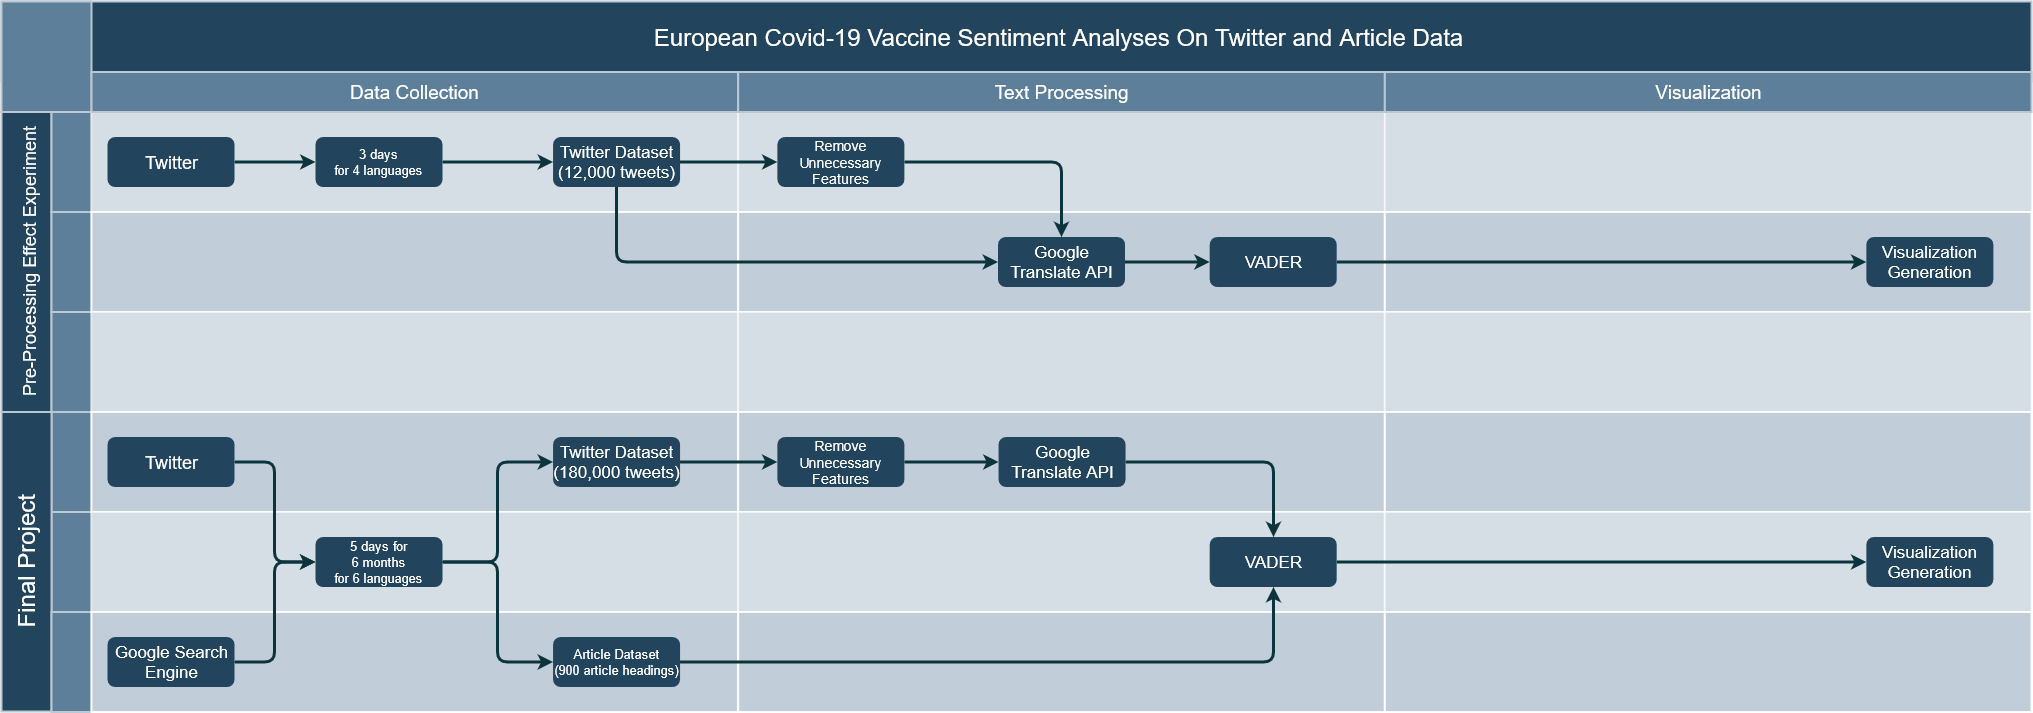
\includegraphics[scale=0.2]{IAPT Flowchart}
\caption[Method Flowchart]{Flowchart of the Method of Experiment\index{Method Flowchart}}
\label{fig:flowchart}
\end{figure}

\section{Data Collection}

\subsection{Twitter Dataset}

The large scale dataset of tweets maintained by \citet{banda2020largescale} is very large and analysing it in its entirety would be expensive, lengthy and out of scope for this \ac{IAPT}, since the majority of the data present is generated outside of the \ac{EU} borders.
The dataset contains daily folders representing each each day from the 22nd of March 2020, which contain two files, one of all tweets and retweets on the day, and the other a cleaned version with no retweets.
Instead all of this available data for every month from December 2020 till May 2021, 5 dates, the 1st, 7th, 14th, 21st, 28th where chosen and the clean dataset file was used.
It was decided that 1000 tweets from 6 languages would suffice to form the Twitter dataset.
The 6 languages, English, Spanish, French, German, Italian and Dutch are the European languages with the most presence in the Panacea Lab dataset.
An important point to consider when using the Panacea Lab dataset is that only the tweet ID is available.
However this ID can be easily used to download and collect the tweet text and other tweet features.
For this \ac{IAPT} the Python library, Tweepy a Python wrapper for the Twitter \ac{API} was used~\citep{roesslein2020tweepy}.
The use of the Twitter \ac{API} requires the signing-up to the service with Twitter, where after approval \ac{API} are shared.
The free version comes with limitations such as a limit of 300 lookups/ 15 minutes, however a limit on status retrieval through the ID does not exist.
Hence for this part of the data collection no limitations were imposed by the Twitter \ac{API}.
In total 180,000 tweets where collected.

A smaller dataset was also collected following the same method as described above.
This smaller dataset features a 1000 tweets from 3 dates, the 1st of January, February and March and 4 languages, English, Spanish, French, German.
This dataset was used to test the effect of pre-processing the tweets before passing them to a \ac{VADER} model.
In total 12,000 tweets where collected.

\subsection{Article Dataset}

As the focus of this \ac{API} was explained to be more directed towards using social media data, it was decided that the article dataset would be much smaller in scale.
Using the Google search engine a query was done for every day a file was taken from the Panacea Lab dataset.
The query was of the format: \\\textquote{{Country} Covid* before:{Date in YYYY-MM-DD Format} After:{Day before Date in YYYY-MM-DD Format}}\\
5 relevant articles where collected for each day and stored in a number of csv files.
In total 900 articles where collected.

\section{Data Processing}

The tweet data collected is unfiltered and contain a number of useless features such as links, stop words and whitespace.
In the first part of this \ac{IAPT} the results of pre-processed tweets and 'naked' tweets are used to create a final pre-process function.
In the final version tweets go through the following process:

\begin{itemize}
    \item HTML special entities (e.g.\ \&amp;) are removed.
    \item Tickers are removed.
    \item Hyperlinks are removed.
    \item Punctuation is removed.
    \item "'s", "'t", "'ve" are split with a space.
    \item Words with 2 or fewer letters are removed.
    \item Whitespace is removed.
    \item Stop words are removed.
\end{itemize}

\noindent The stop word list for the various languages where taken from the \ac{NLTK}~\citep{bird2009natural} library.
Article headings in the article dataset do not go through this pre-processing step.

For translation, non-English pre-processed tweet text was passed sent to the Google Cloud Translation \ac{API}.
The total cost of using the translation \ac{API} came to €60.
Article headings where not translated as they where collected only in English.

\section{Sentiment Analyses}

The \ac{NLTK}~\citep{bird2009natural} library was employed to implement a \ac{VADER}~\citep{Hutto_Gilbert_2014} model.
Each tweet and article heading was used as an input and the compound \ac{SA} score was kept.
The mean compound score of each day was stored in a file, while each score was classifies as either:

\begin{itemize}
    \item very positive (score >= 0.75)
    \item positive (0.25 <= score < 0.75)
    \item neutral (-0.25 <= score < 0.25)
    \item negative (-0.75 <= score < 0.25)
    \item very negative (score < -0.75)
\end{itemize}

\section{Visualization}

The \ca{SA} scores where visualized with the use of the Multiplex~\citep{Mamo2021} library and the matplotlib library~\citep{Hunter:2007} via the use of Time Series plots and word clouds for each month.
A word cloud visualization was also generated for every language (translated to English) for every month.
The focus of these visualizations was aimed at the results stemming from the Twitter dataset.
Discussion on the visualizations produced are found in the following chapter, Results \& Discussion.
    \chapter{Results \& Discussion}
%\textbf{Should include a reiteration of the experiments, and their outcome.  Together with a description (discussion).  Preamble should include a reminder of the aims and objectives together with a list of experiments to achieve these.  Should include many charts and other visualization with appropriate descriptions}.

\section{Data Collection Validation}

In the pre-processing experiment, the method used for collecting and filtering the 1000 Tweets.
To test that the distribution and collection was being done correctly, figures~\ref{fig:preprocessdist} and~\ref{fig:finaldist} where generated.


\begin{figure}[!htb]
\minipage{0.5\textwidth}
  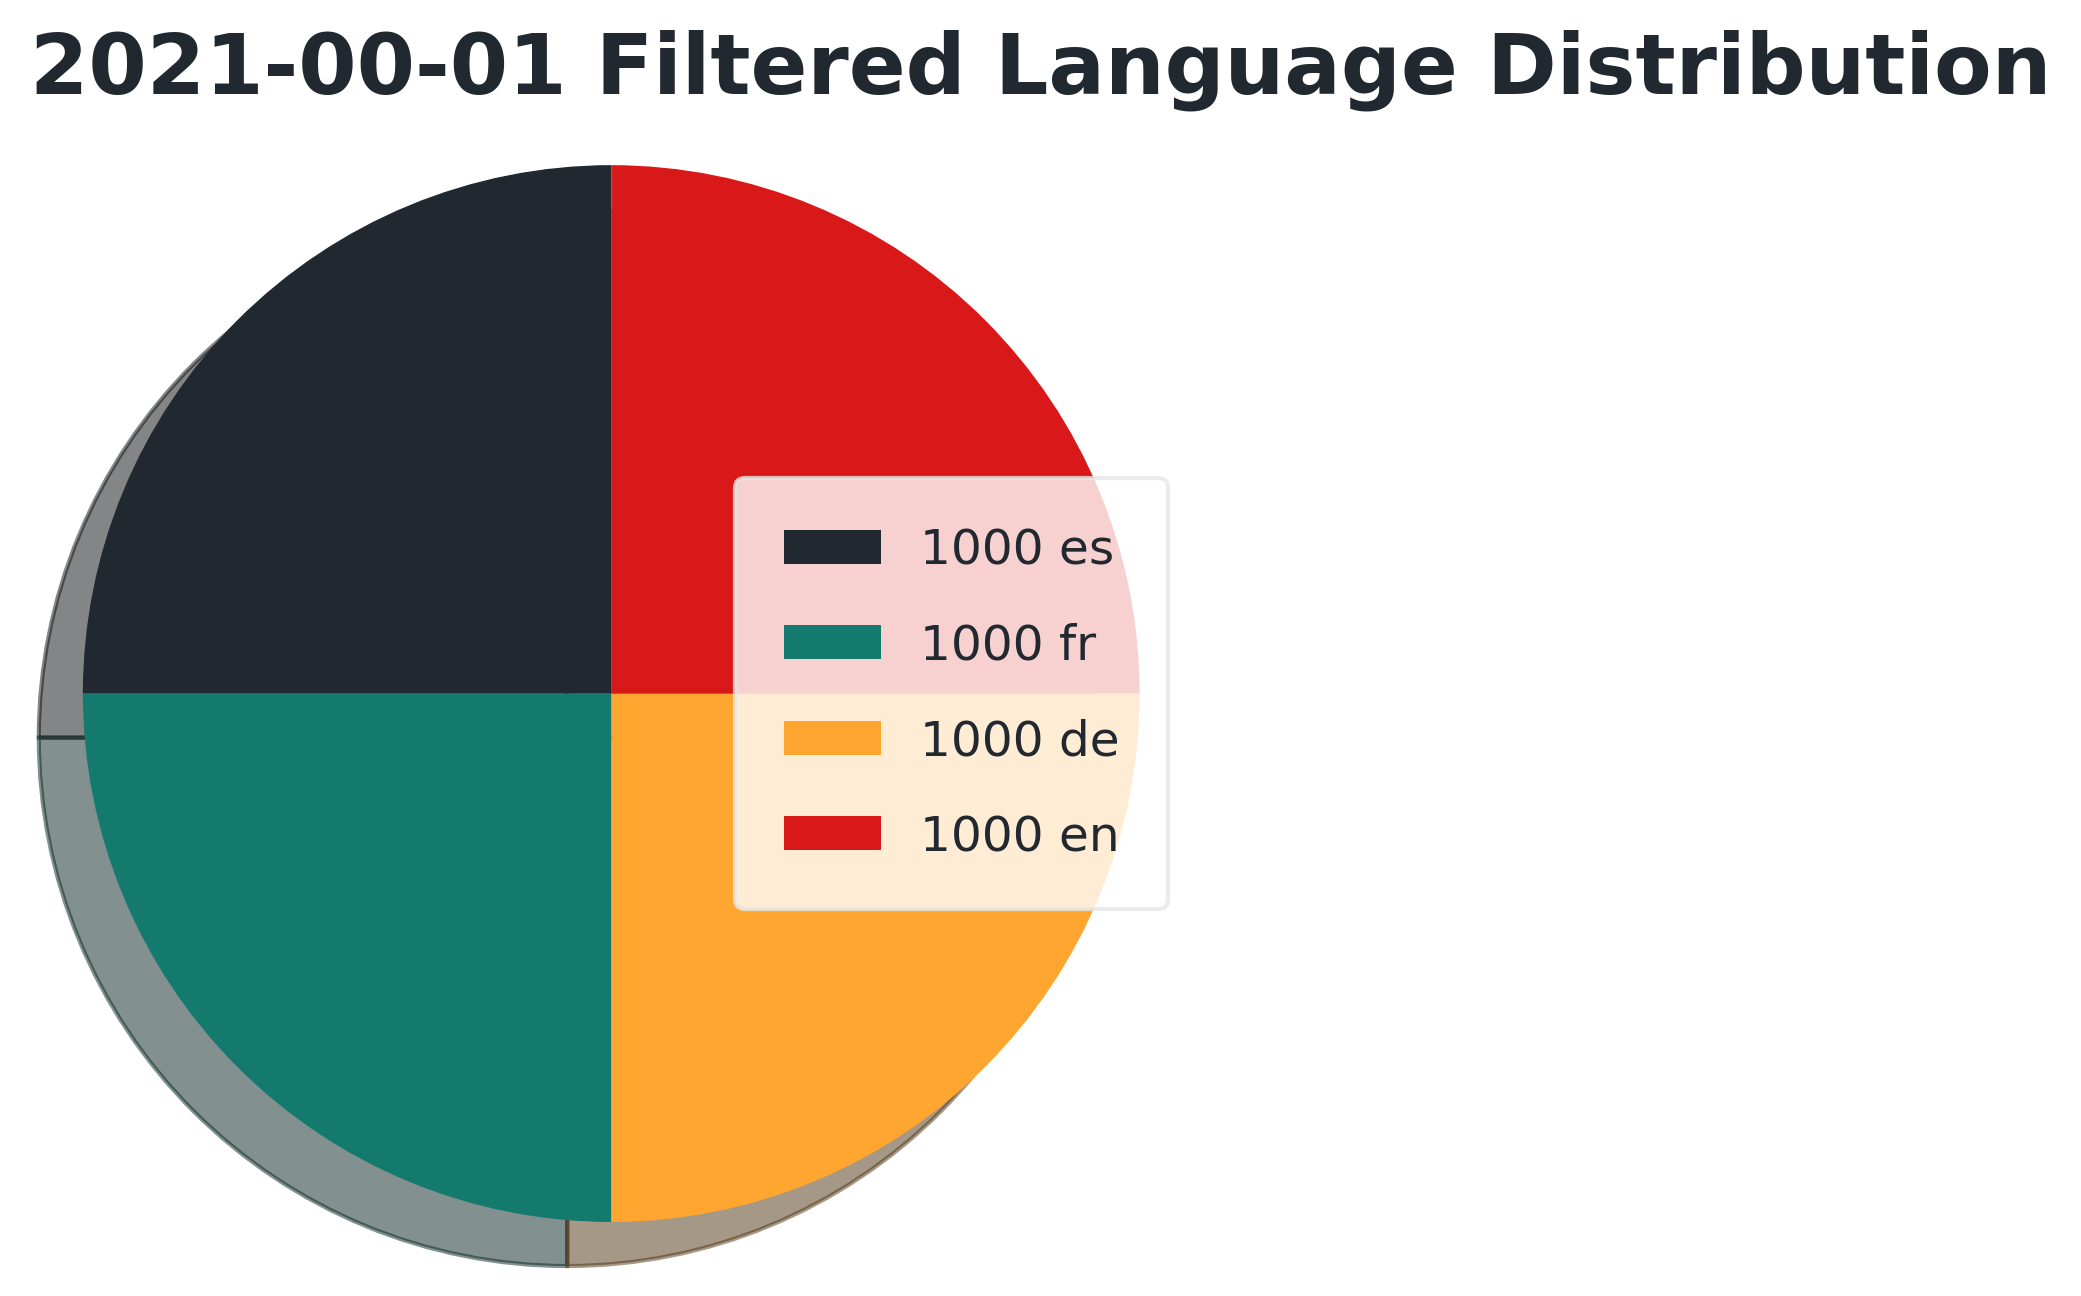
\includegraphics[width=\linewidth]{2021-00-01 Filtered Language Distribution.png}
  \caption[Pre-Process Filtered Language Distribution]{ }
  \label{fig:preprocessdist}
\endminipage\hfill
\minipage{0.5\textwidth}
  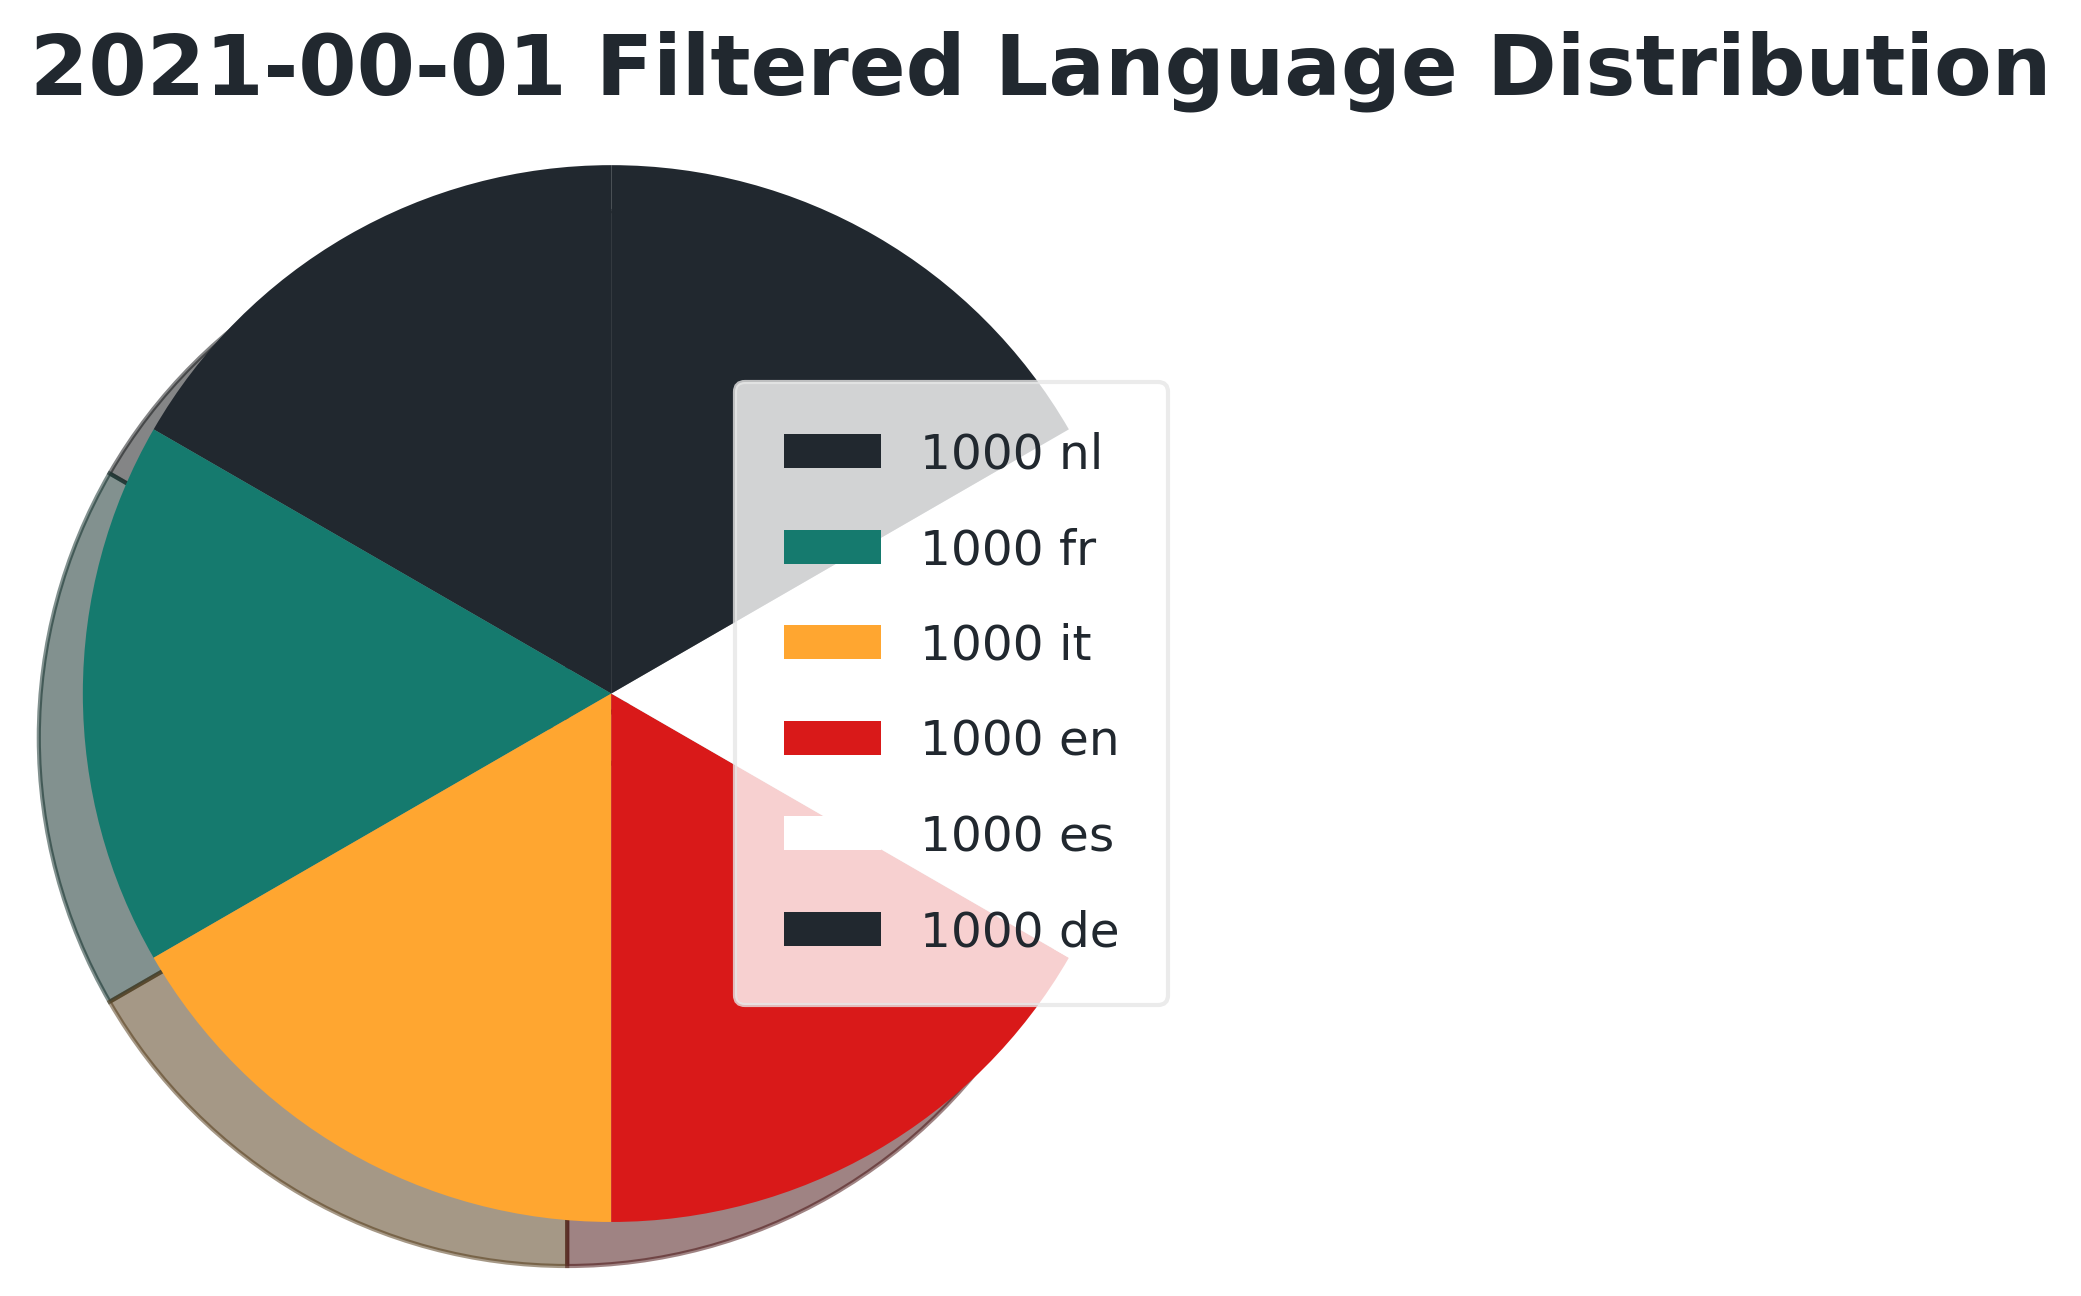
\includegraphics[width=\linewidth]{2021-01-01 Filtered Language Distribution - Final.png}
  \caption[Final Filtered Language Distribution]{ }
  \label{fig:finaldist}
\endminipage
\end{figure}


\section{Pre-Processing Effect}

The compound sentiment scores returned from the \ac{VADER} model was averaged and plotted for the 3 dates used in the experiment.
The 4 graphs produced, figures~\ref{fig:EnglishPre} to~\ref{fig:GermanPre}, show a time series graph of each language over the 3 days which are 1 month apart.
The mean scores where also summed and the difference between the pre-processed and non-processed total was of 0.17\%.

\begin{figure}[!htb]
\minipage{0.5\textwidth}
  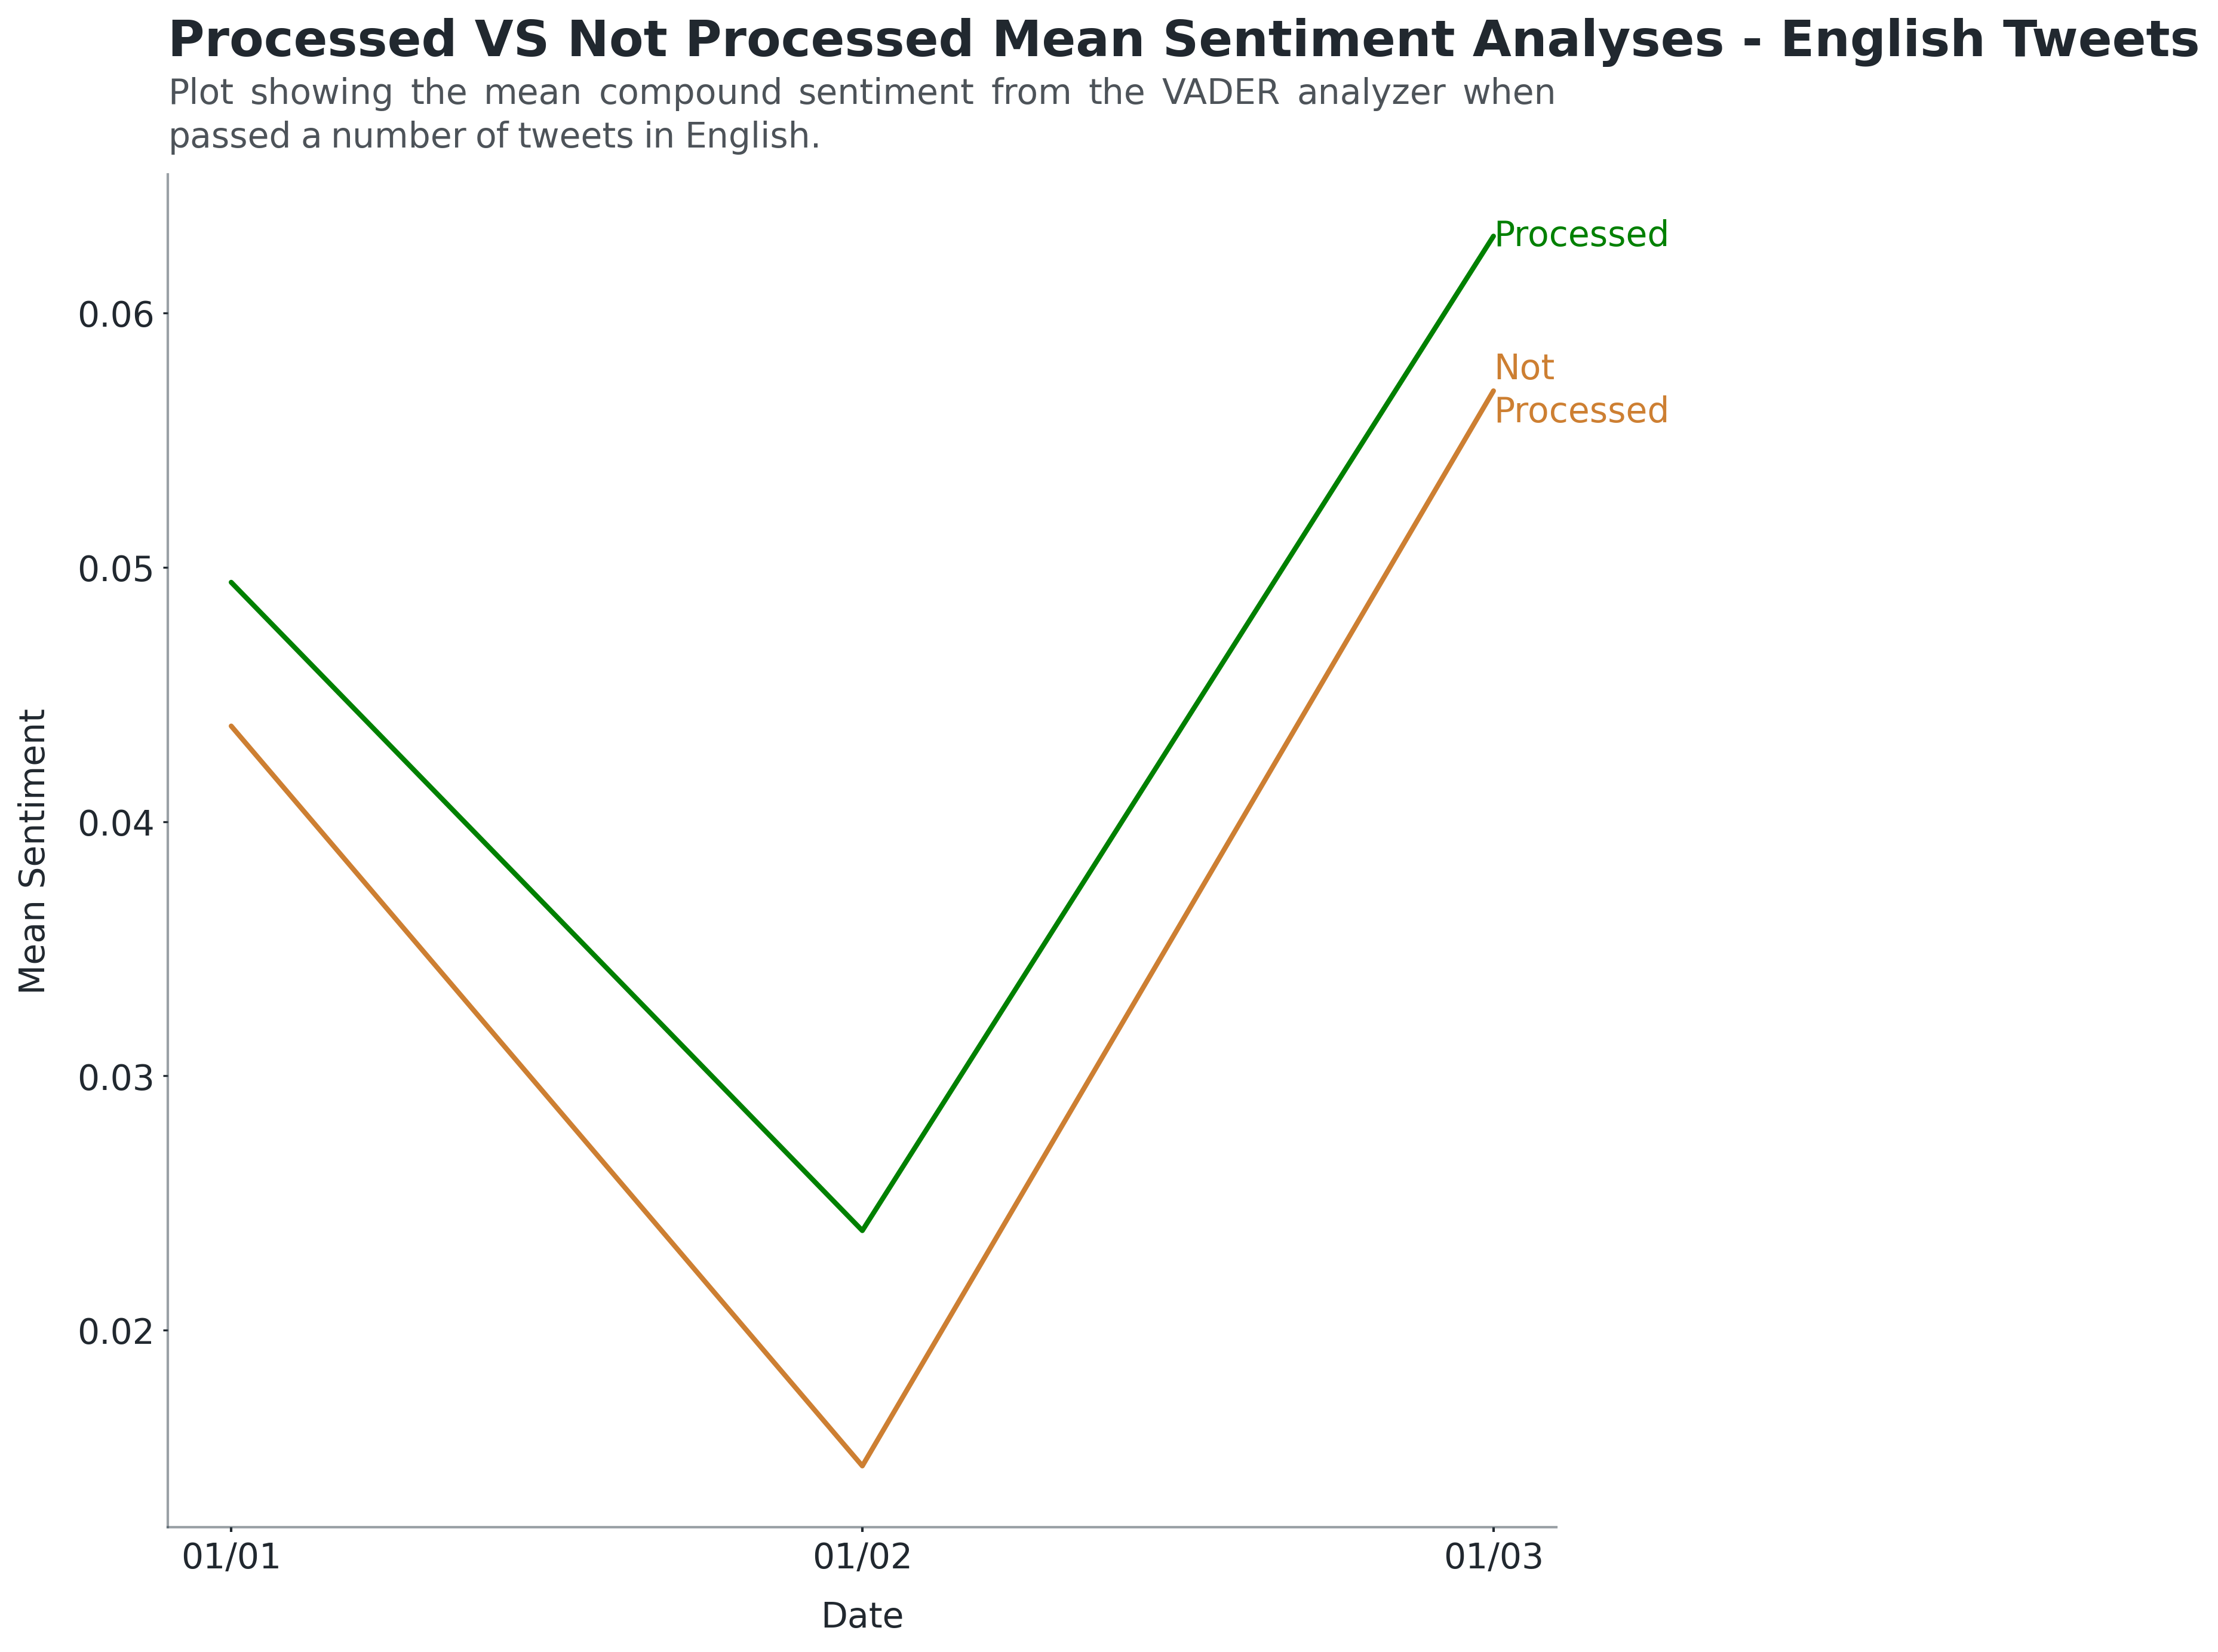
\includegraphics[width=\linewidth]{English Process VS NotProcessed.png}
  \caption[English Process VS NotProcessed]{ }\label{fig:EnglishPre}
\endminipage\hfill
\minipage{0.5\textwidth}
  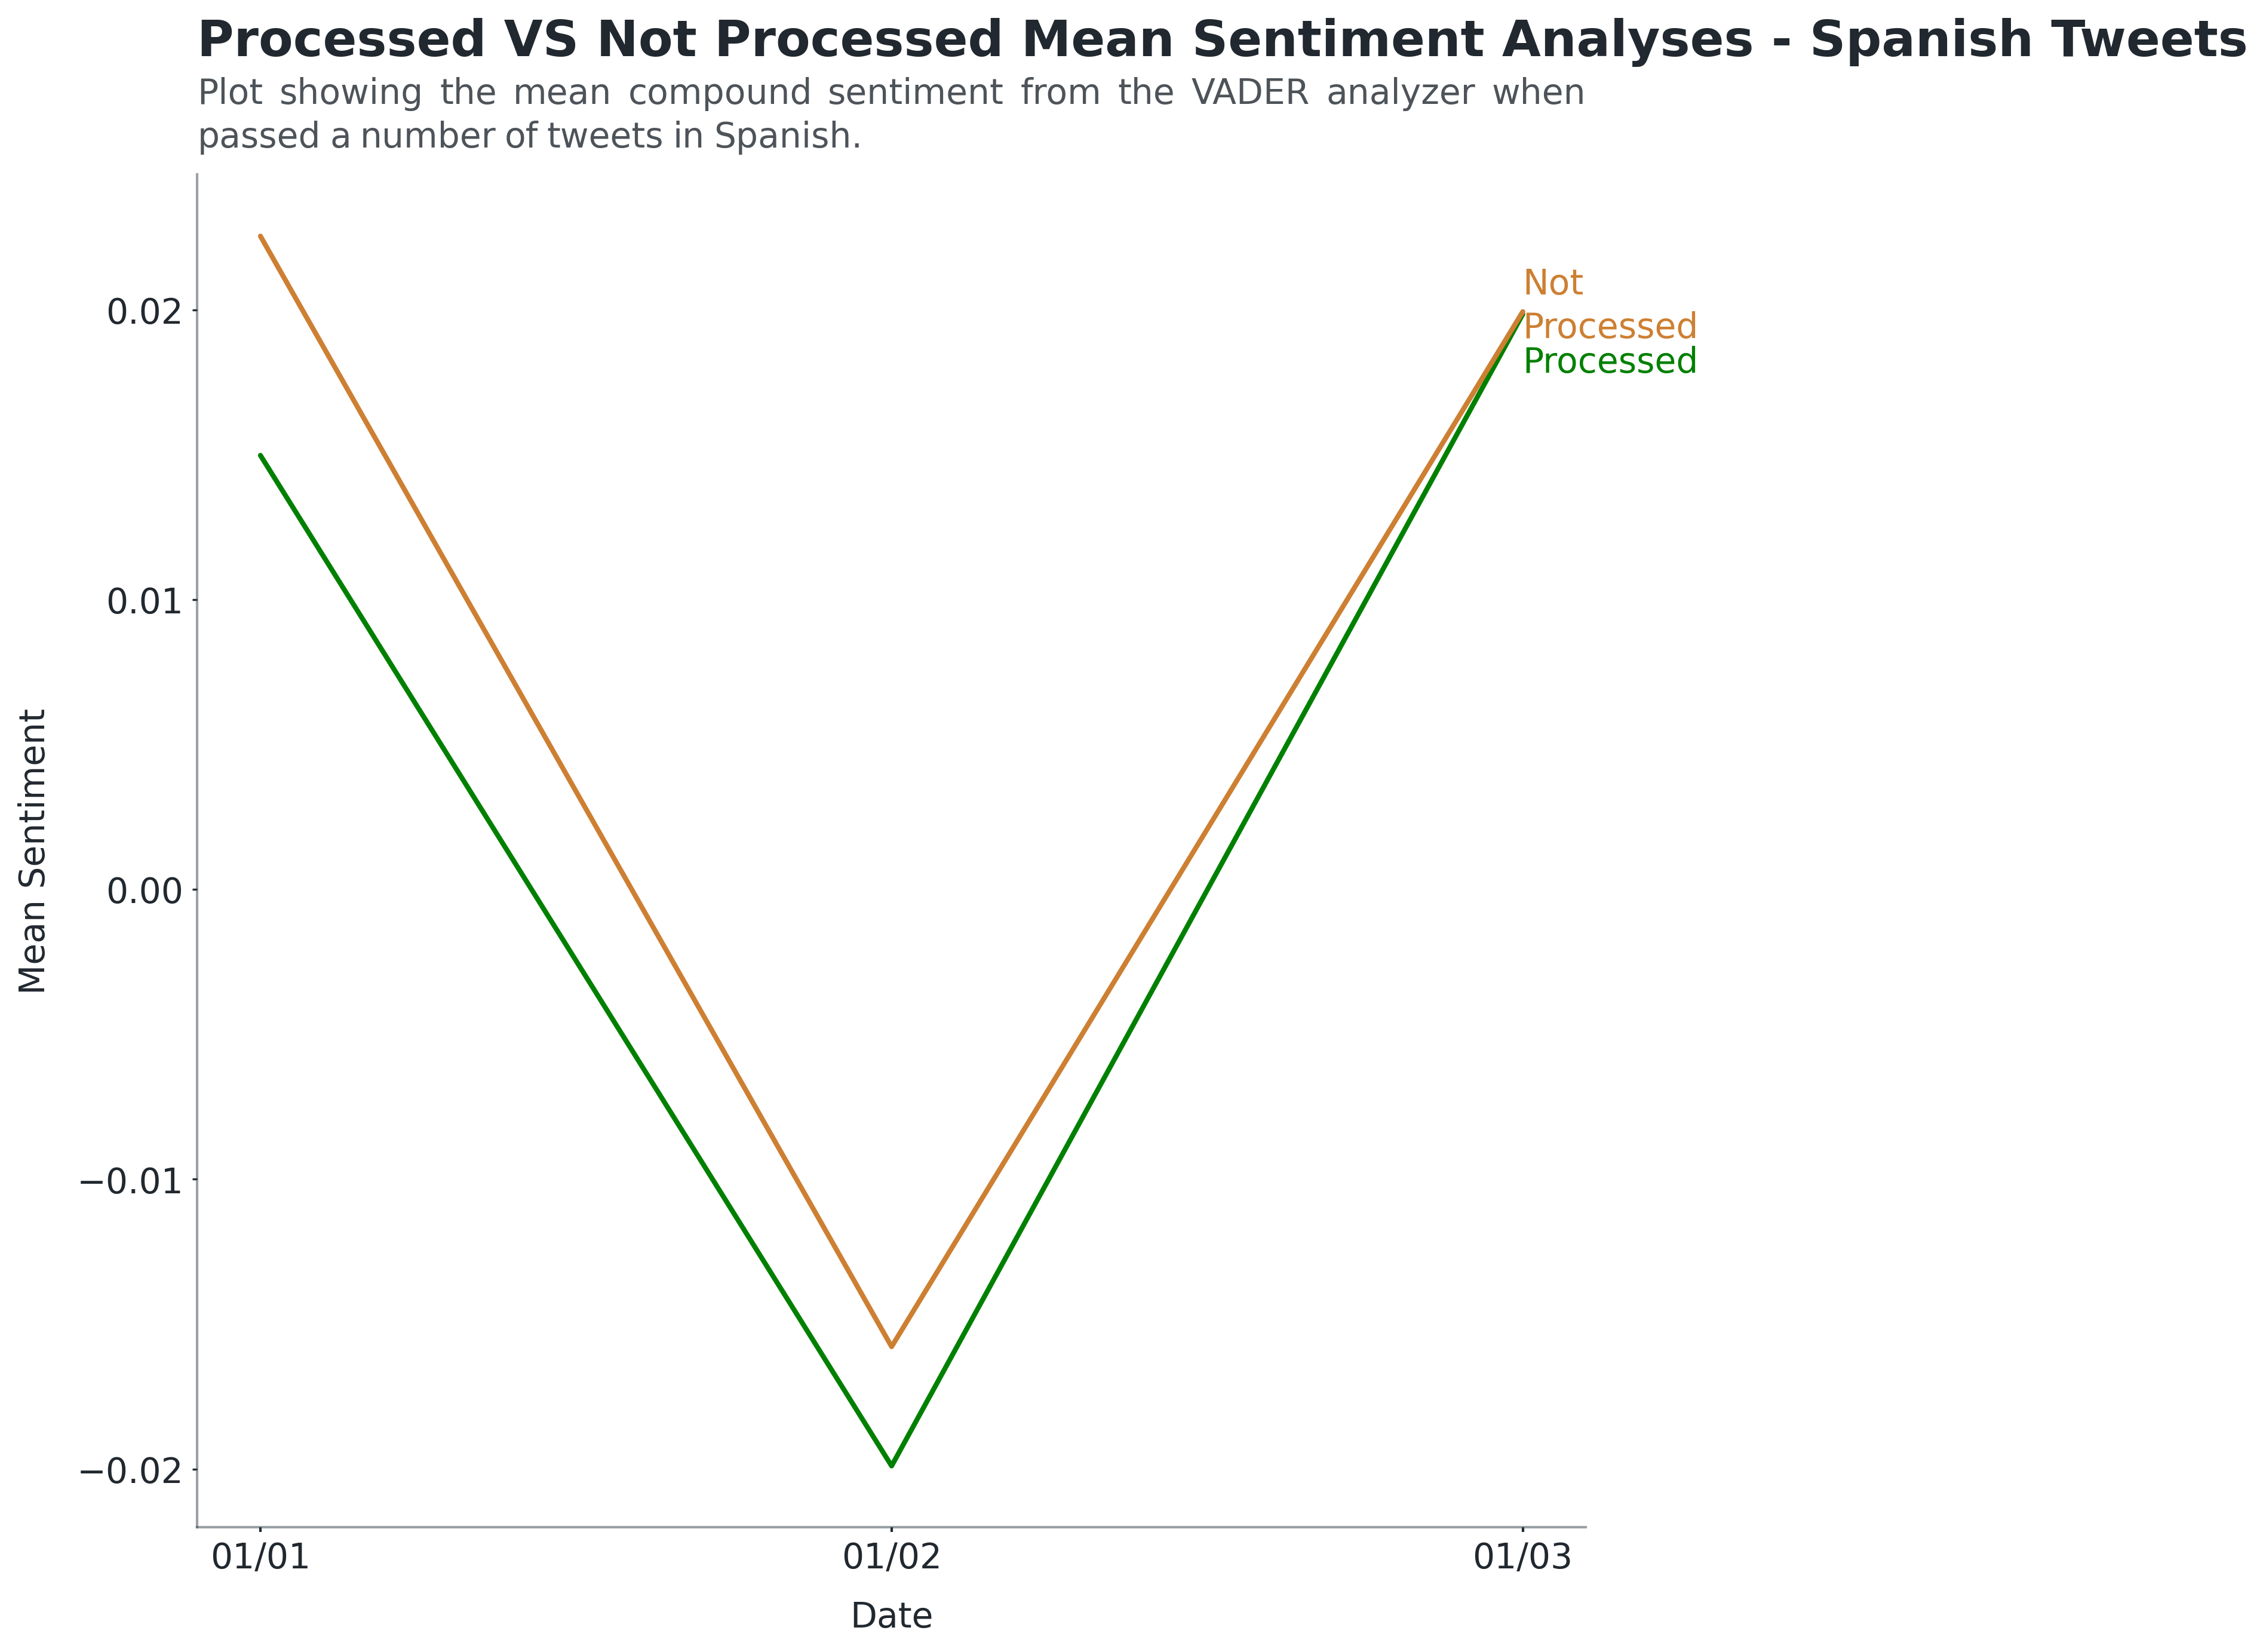
\includegraphics[width=\linewidth]{Spanish Process VS NotProcessed.png}
  \caption[Spanish Process VS NotProcessed]{ }\label{fig:SpanishPre}
\endminipage
\end{figure}
\begin{figure}[!htb]
\minipage{0.5\textwidth}
  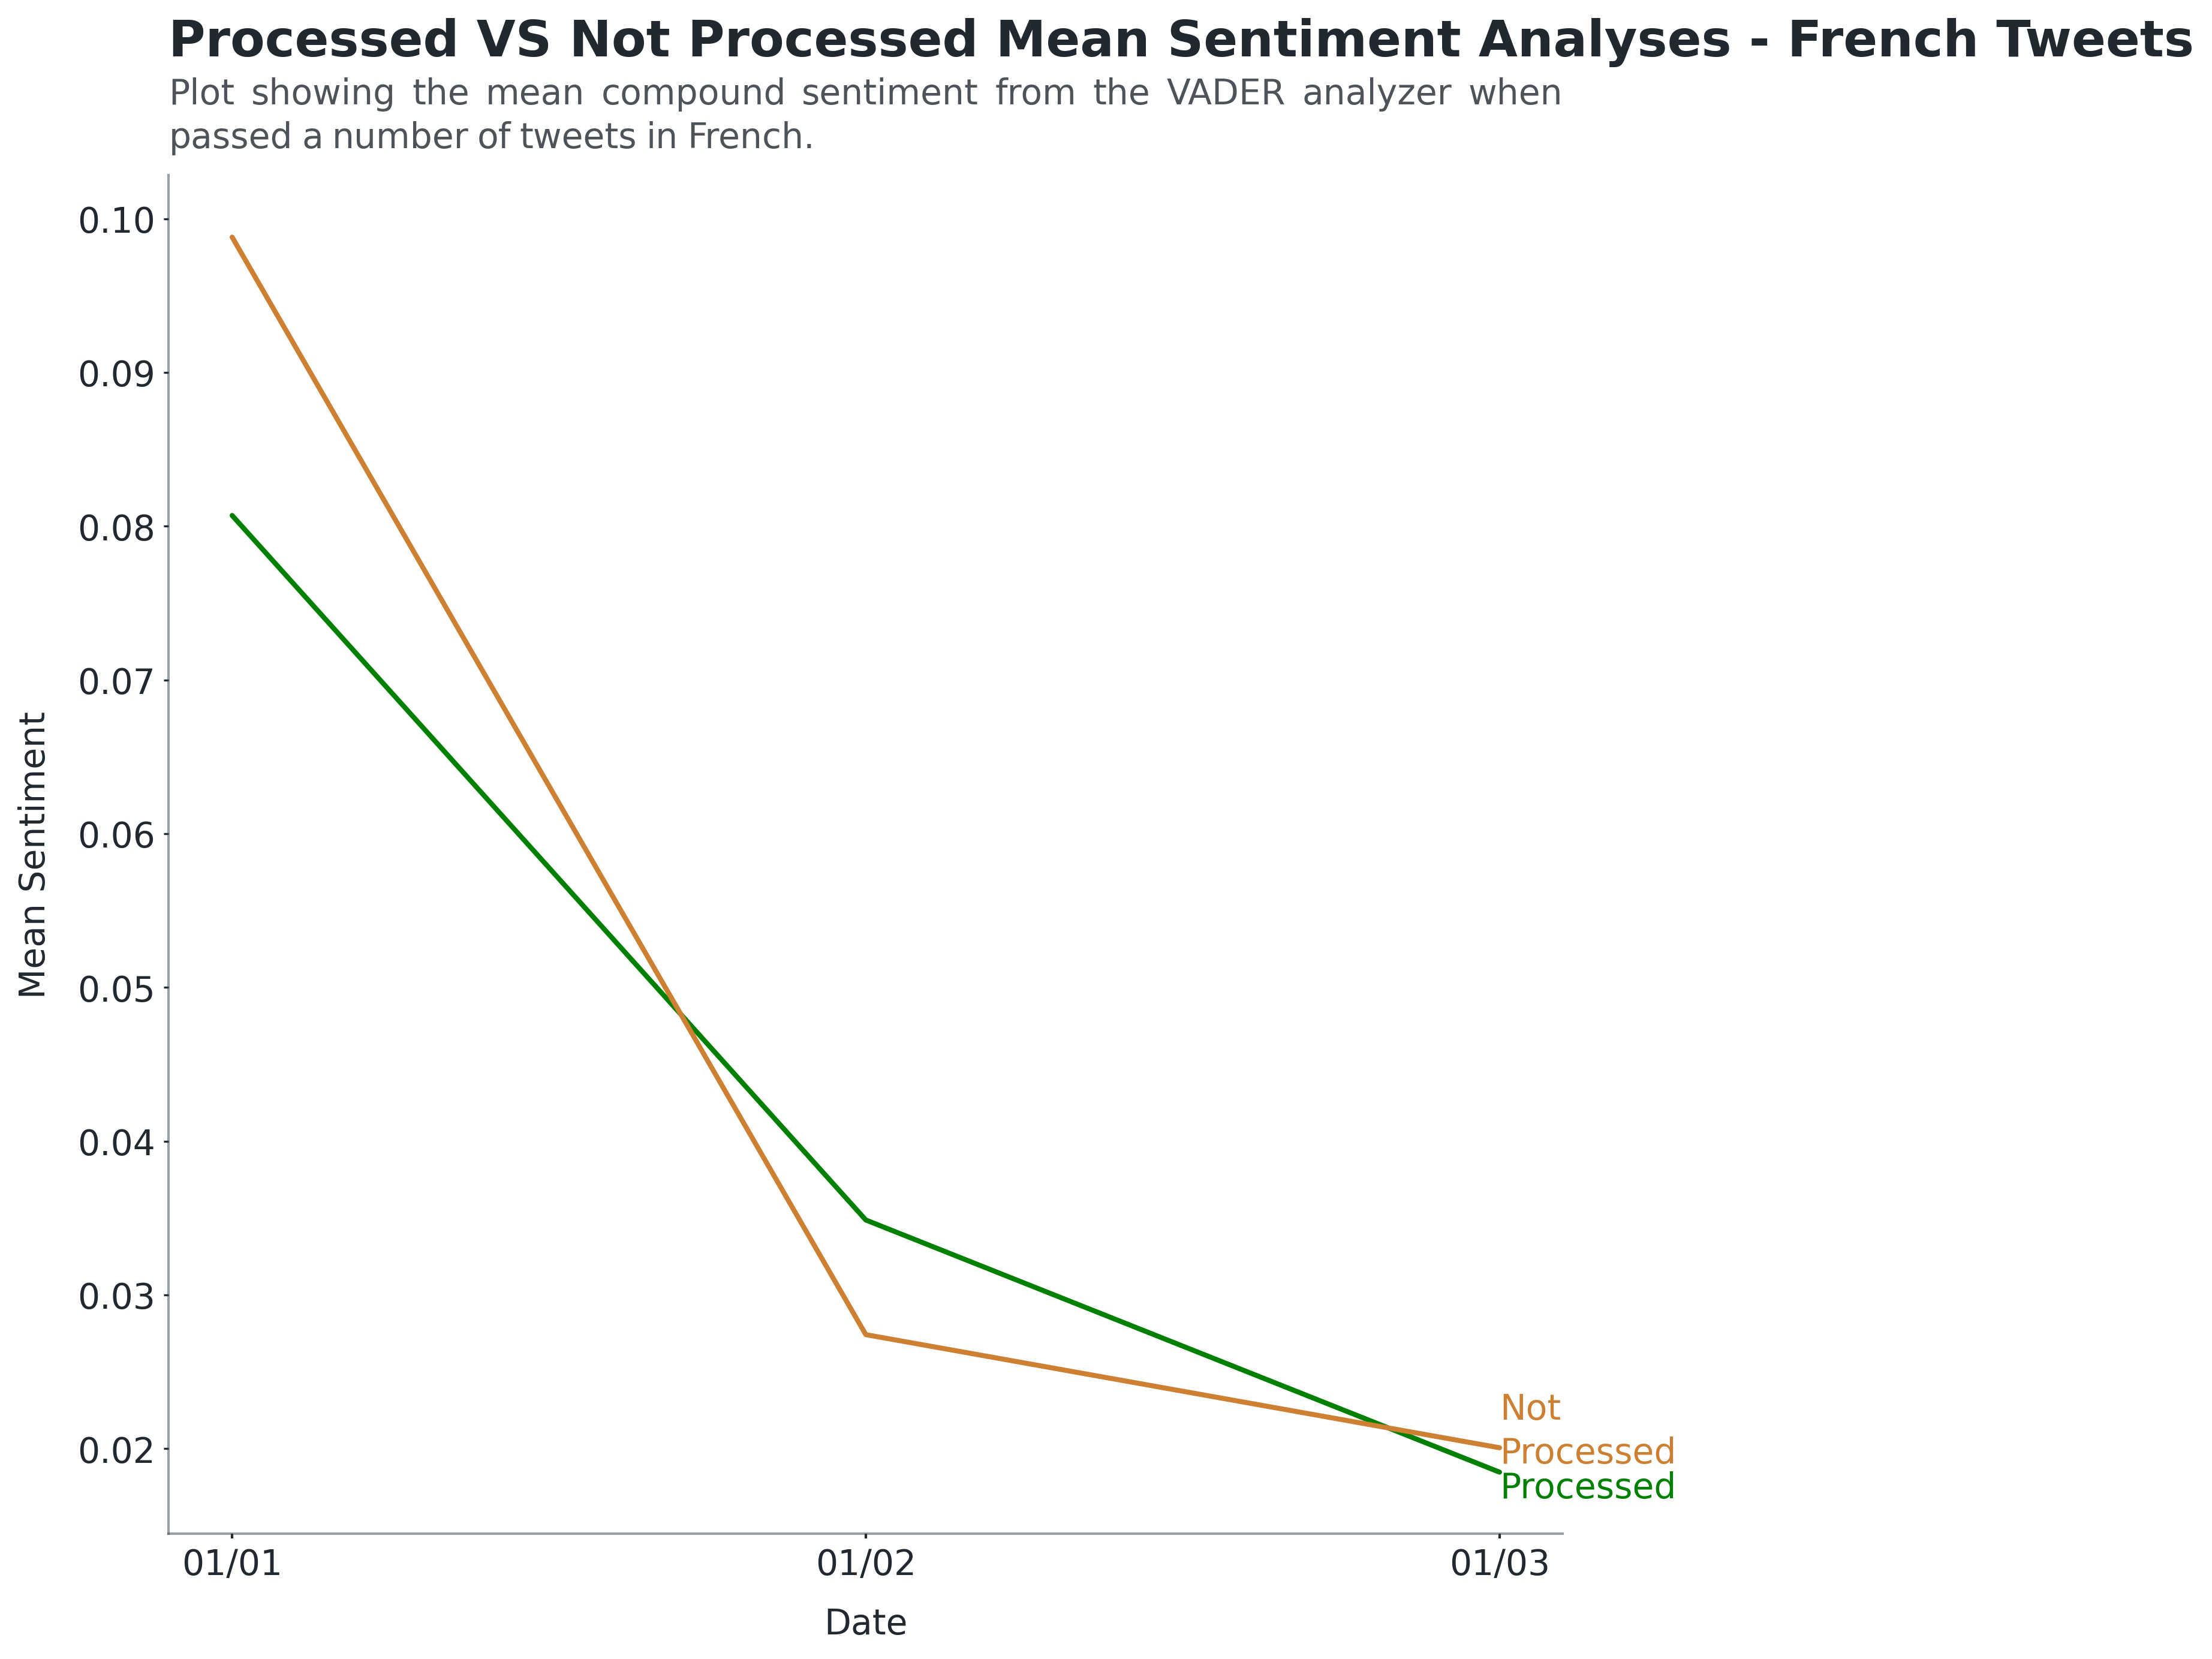
\includegraphics[width=\linewidth]{French Process VS NotProcessed.png}
  \caption[French Process VS NotProcessed]{ }\label{fig:FrenchPre}
\endminipage\hfill
\minipage{0.5\textwidth}
  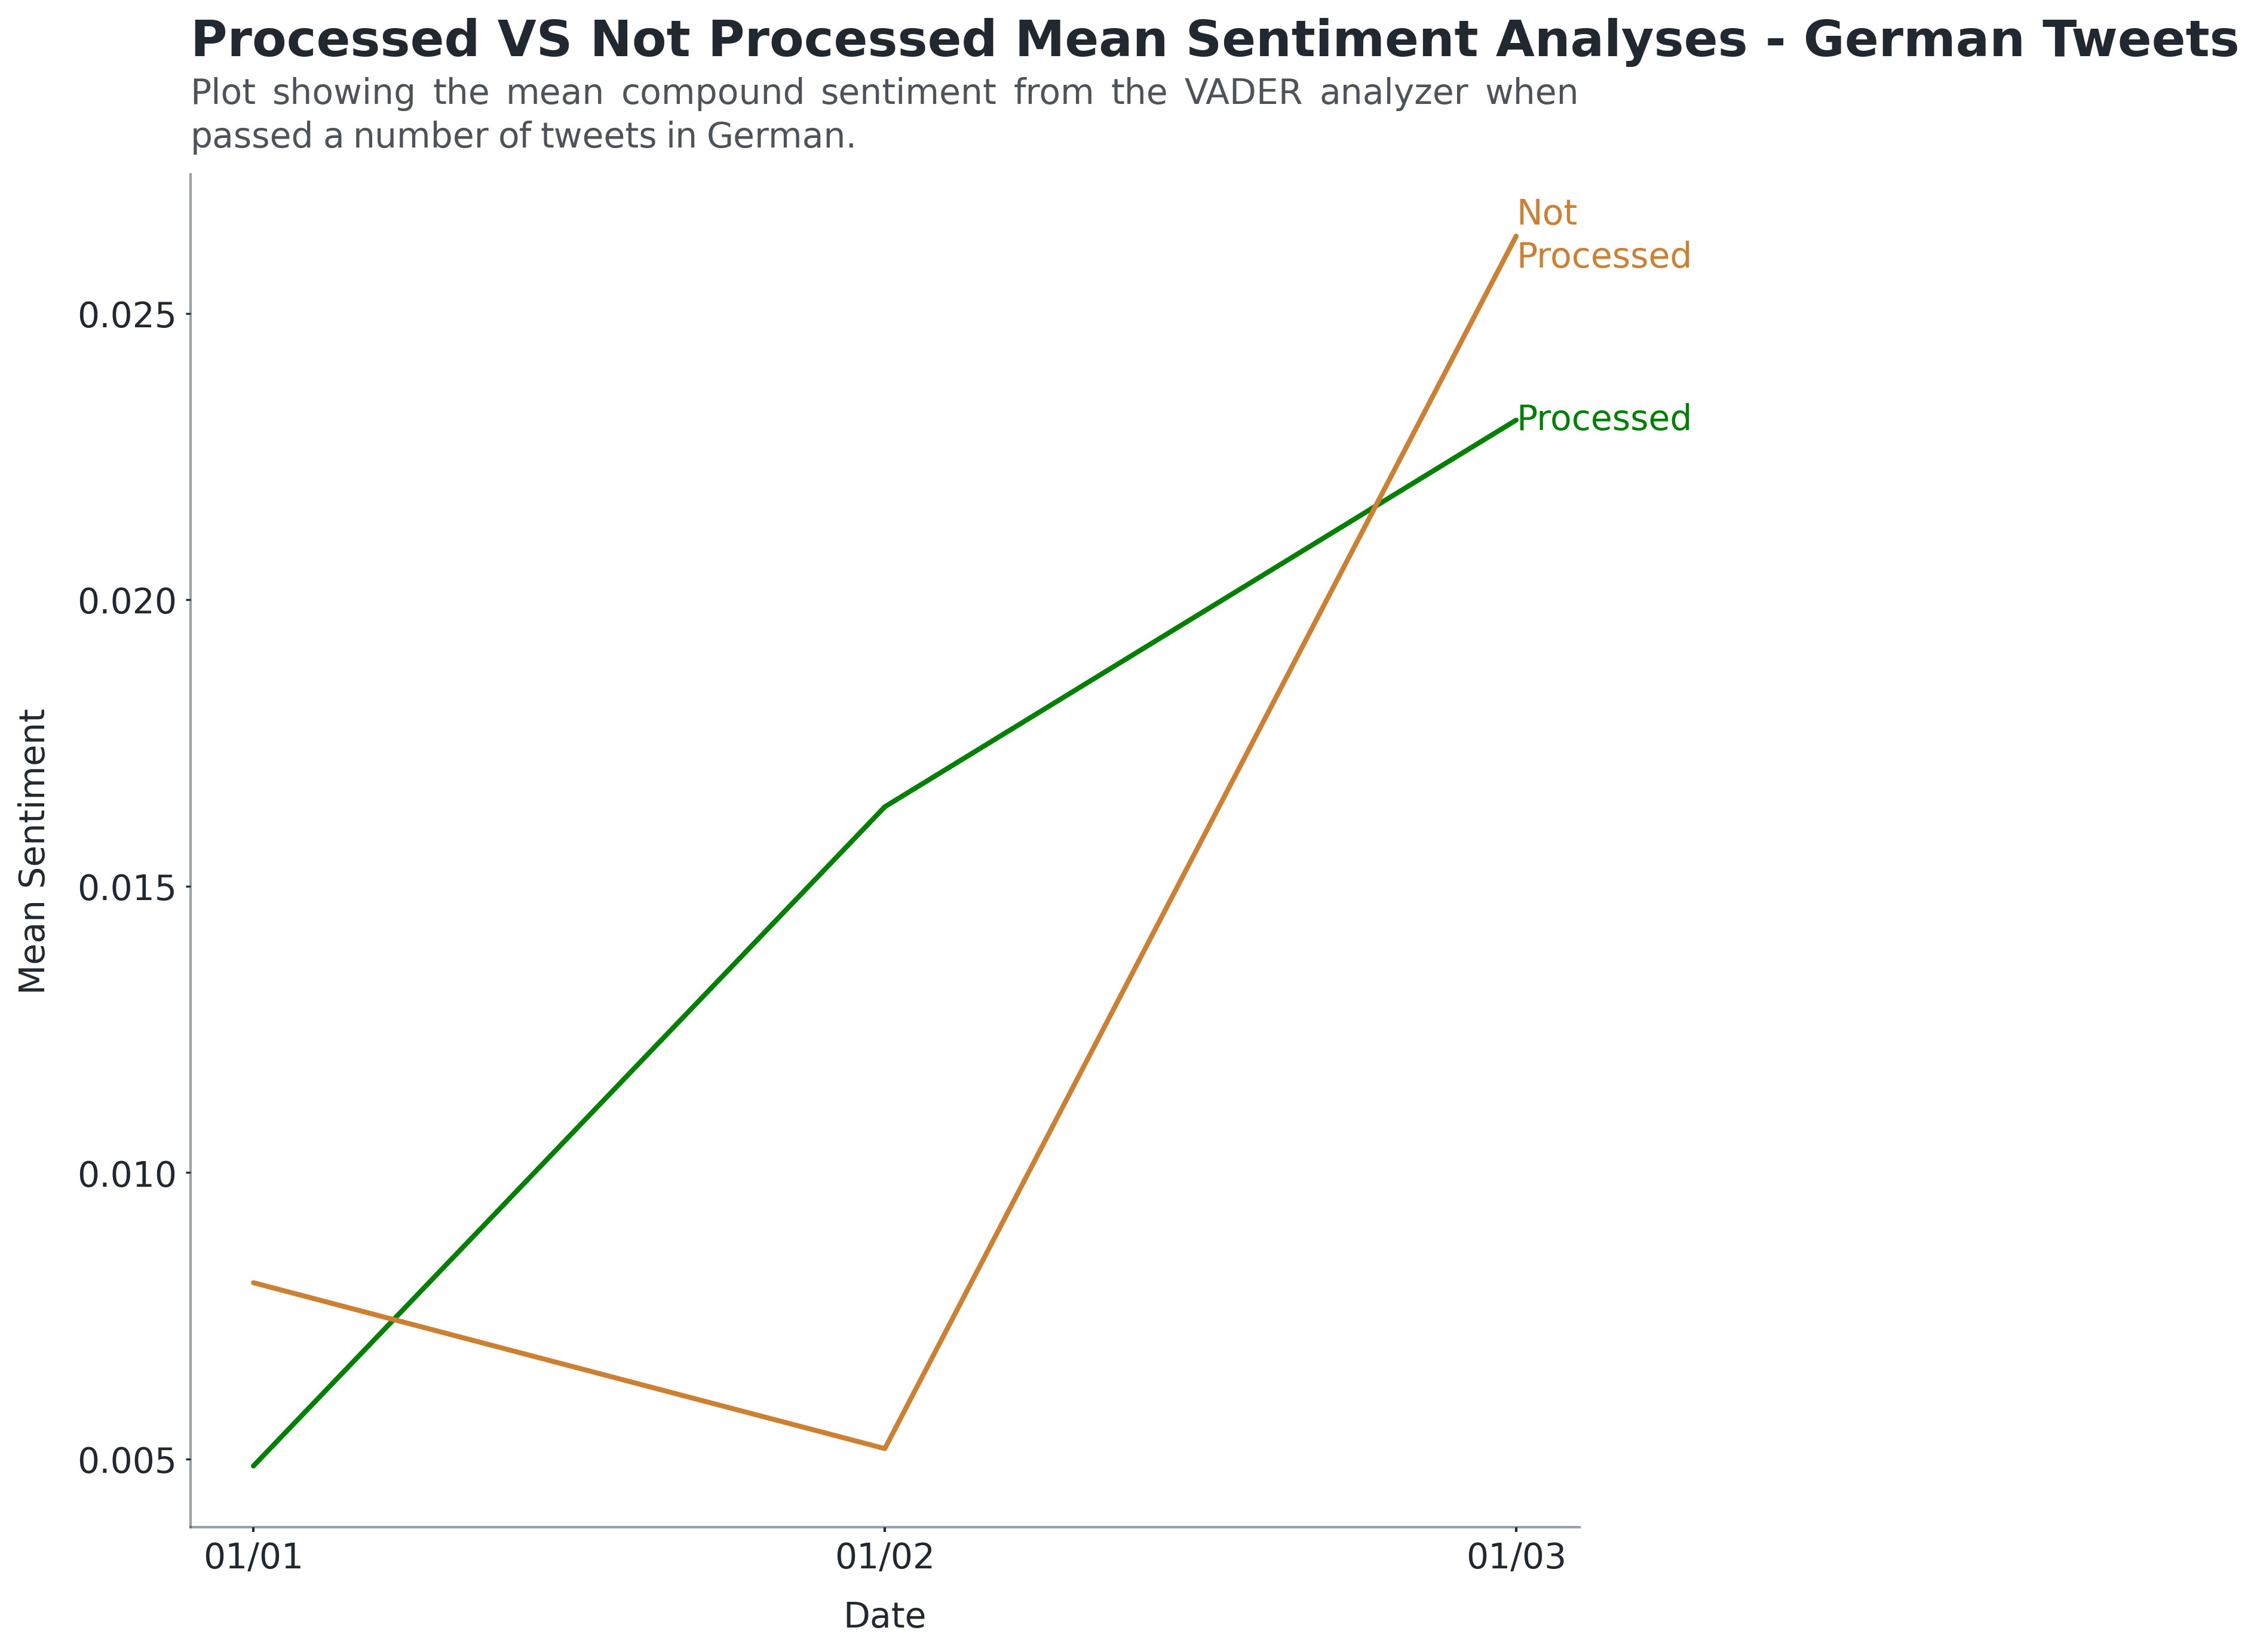
\includegraphics[width=\linewidth]{German Process VS NotProcessed.png}
  \caption[German Process VS NotProcessed]{ }\label{fig:GermanPre}
\endminipage
\end{figure}

\noindent The difference calculated along with the shapes of the graphs plotted were not considered significant enough to remove pre-processing.
However the pre-process function was amended to keep more features like emojis and hashtags, which prior to this experiment where being removed.

\section{Daily Twitter Mean Sentiment}

Just as with figures~\ref{fig:EnglishPre} to~\ref{fig:GermanPre}, time series graphs where plotted for the mean sentiment scores on the larger 180,000 tweet dataset.
When all the languages are plotted against each other in figure~\ref{fig:globalall} show no clear trend, however some languages are closer to each other than others.
When these languages are separated in figures~\ref{fig:globalmean} and~\ref{fig:globaleu} the mean of the compound scores can be seen to related more to each other.

\begin{figure}[h!]
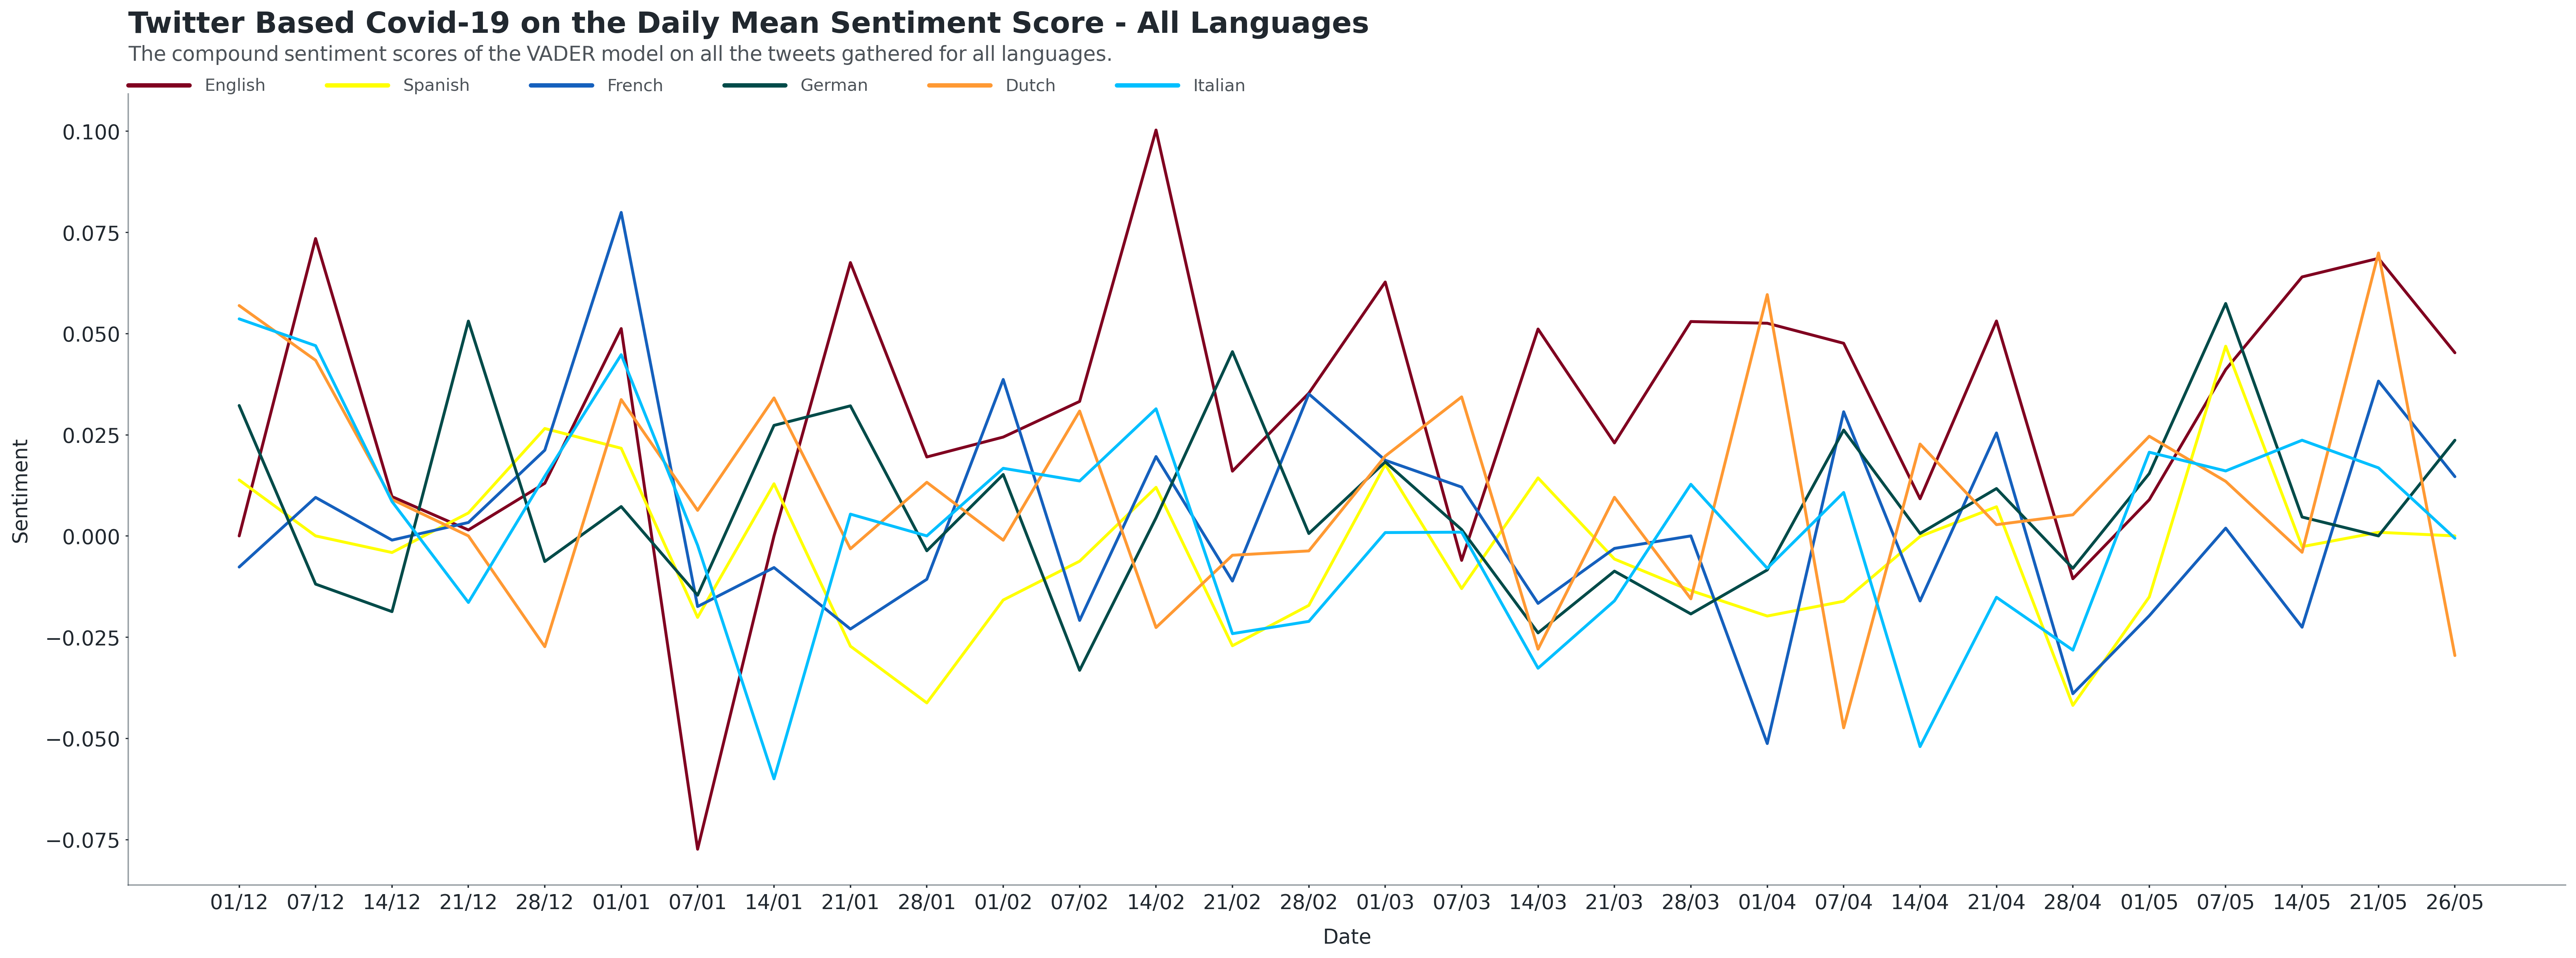
\includegraphics[scale=0.3]{Daily Mean All.png}
\caption[Daily Mean All]{ }
\label{fig:globalall}
\end{figure}

\noindent The effect of translation is very apparent with the reduced information given from the lines plotted from non-English tweets.

\begin{figure}[h!]
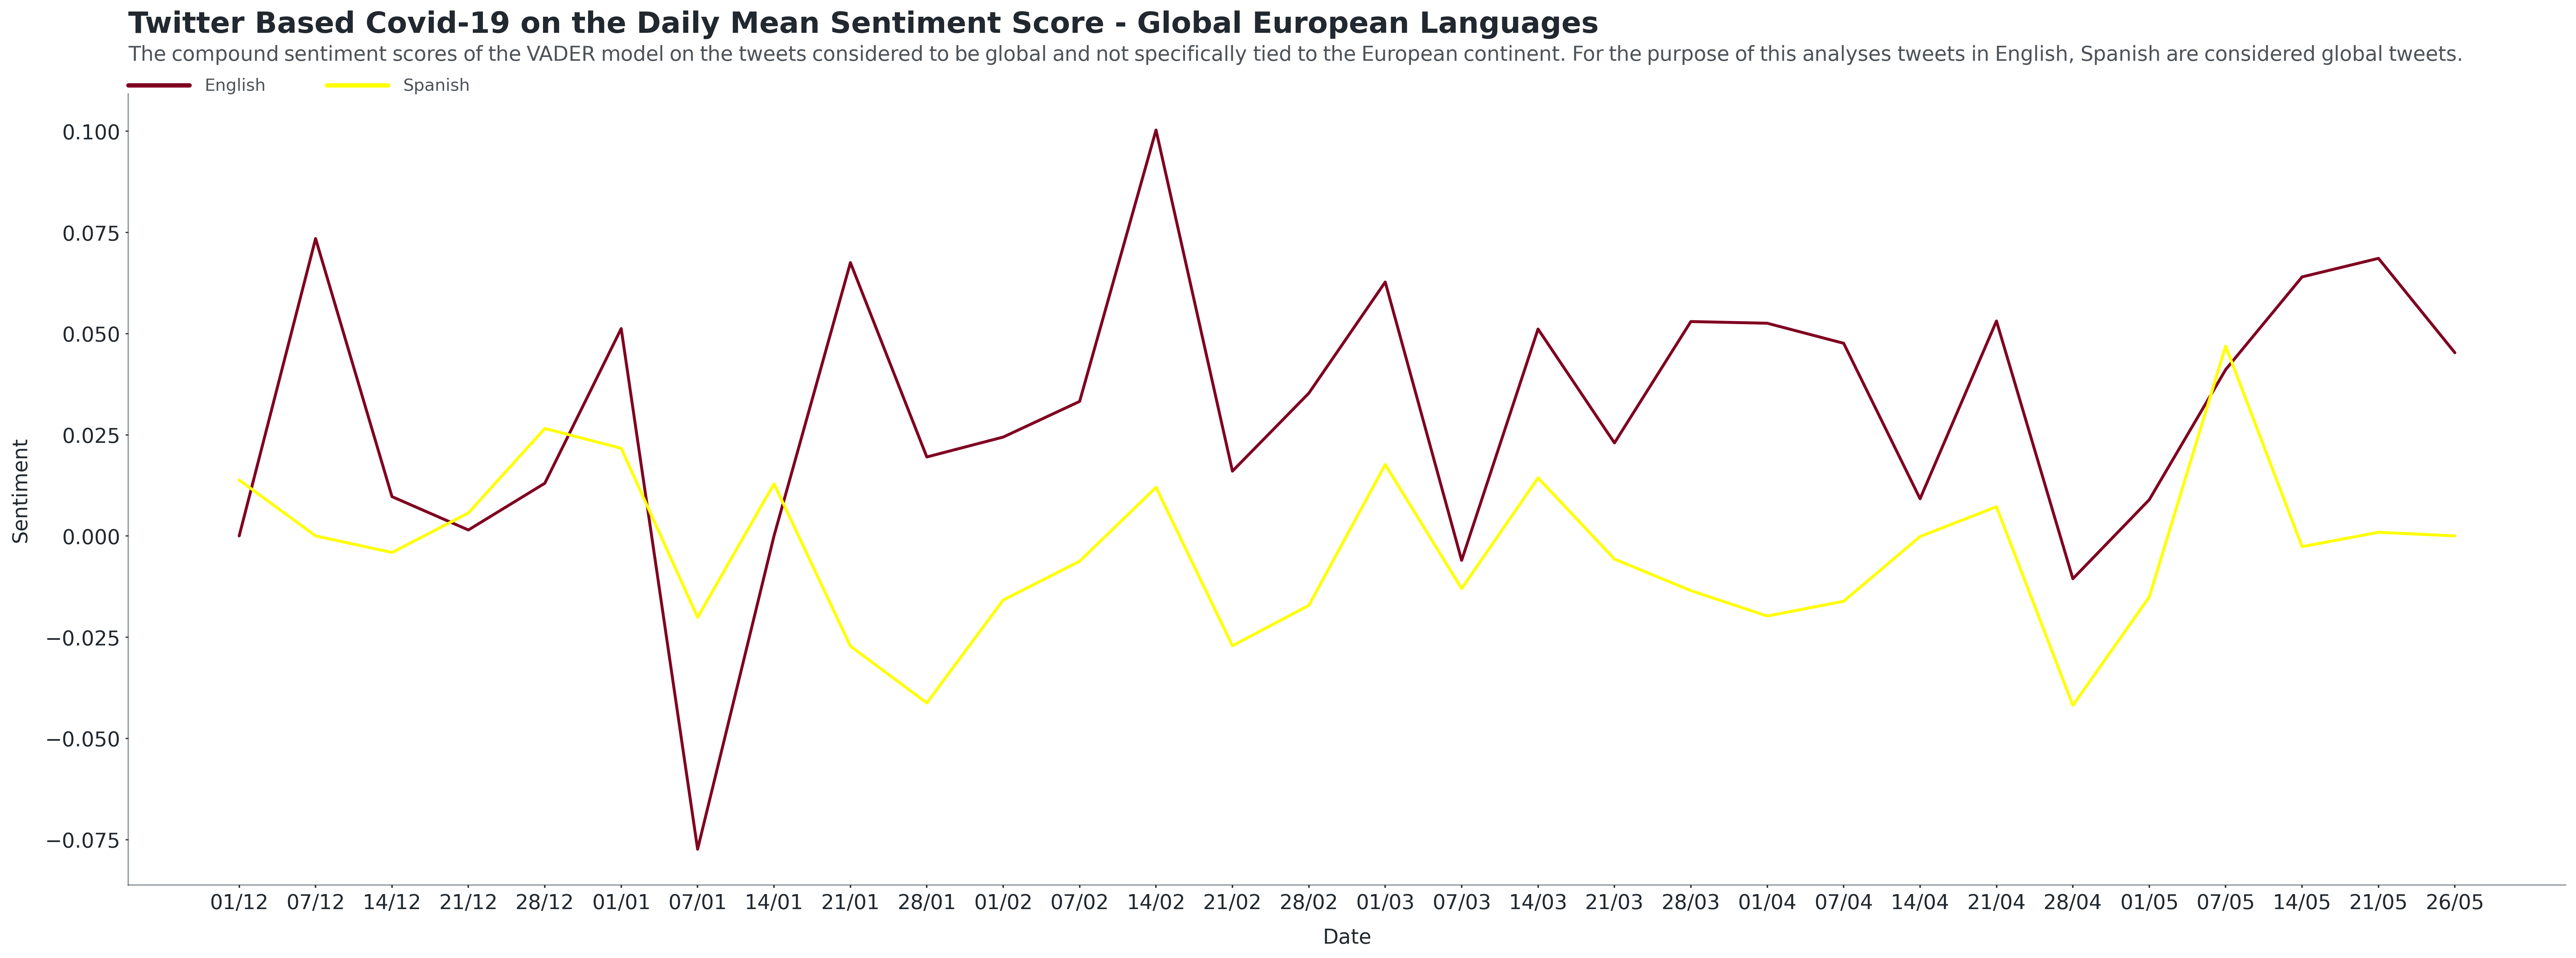
\includegraphics[scale=0.3]{Daily Mean Global.png}
\caption[Daily Mean Global]{ }
\label{fig:globalmean}
\end{figure}

\noindent Although not followed exactly, the shape of the Spanish line corresponds to the peaks and dips of the English line.

\begin{figure}[h!]
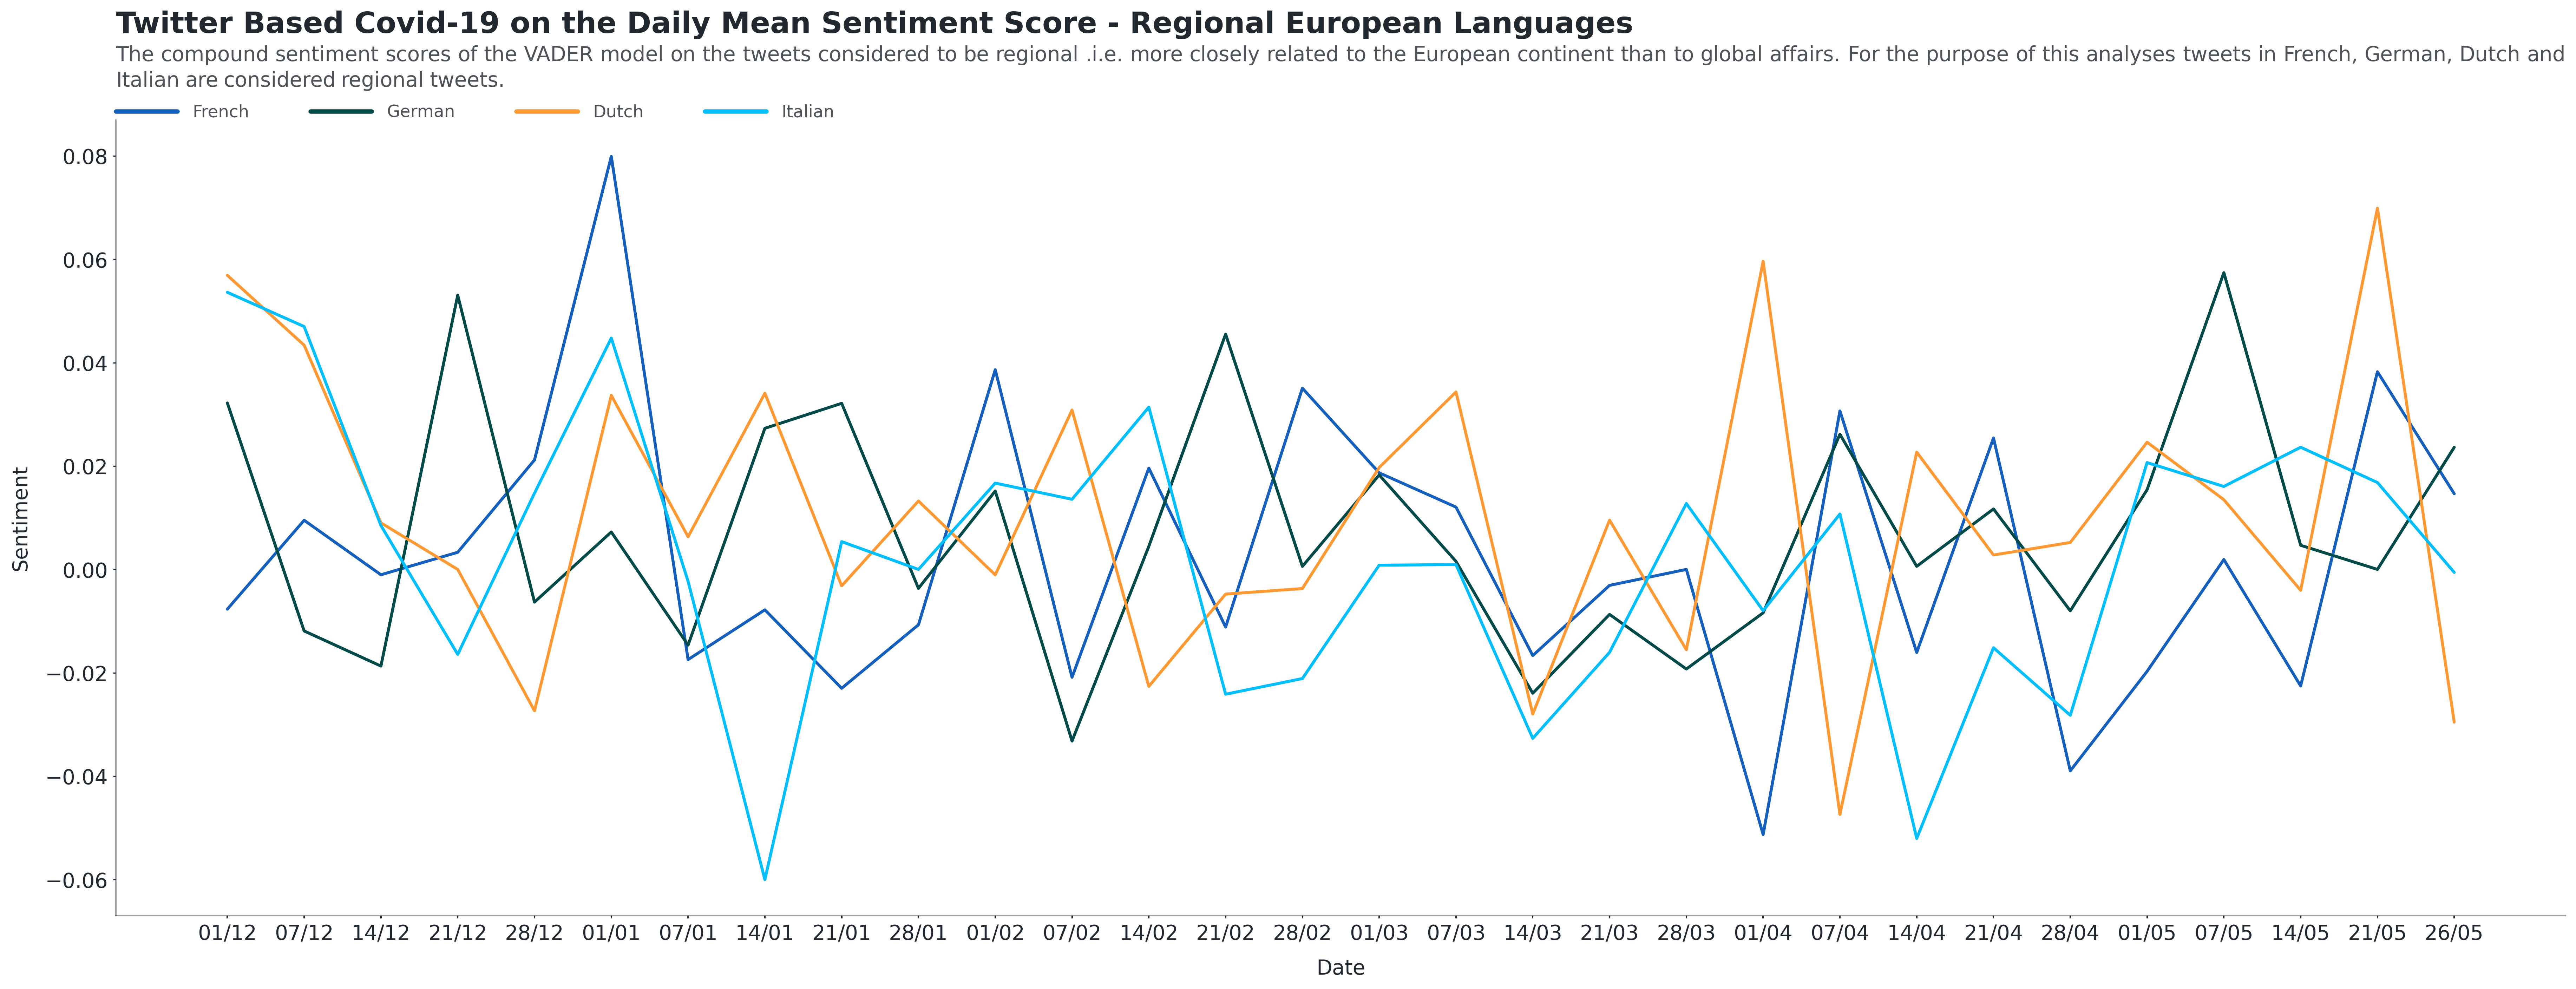
\includegraphics[scale=0.3]{Daily Mean Europe.png}
\caption[Daily Mean Europe]{ }
\label{fig:globaleu}
\end{figure}

\noindent The line plots for these languages where expected to be more closely related however some similarities can be seen.
On holidays such as 1st January (new years) or 14th February(valentines day) most countries experience a peak in positivity.
Inversely on the 14th March every country experienced a dip in positivity.

\section{Daily Twitter Sentiment Classification}



\section{Daily Article vs Twitter Mean Sentiment}



\section{Daily Twitter Sentiment Classification with Article Mean Sentiment}



\section{Word Frequency in the Form of Word Clouds}


    \chapter{Evaluation}

%\textbf{In an ideal world, you should have two kind of evaluations.  The first is against some ground truth (perhaps a random model?).  The second kind of evaluation is against other people's work (accuracy, speed, etc.).  Any dimension which is of interest, should be evaluated.  Evaluation should be statistically sound. }

The methods used for this \ac{IAPT} do not result an objective value.
In fact the scope was to view and analyze the publicly available Twitter user generated, and as explained earlier this data is completely subjective to the user generating it.
However through the use of \ac{SA} and the \ac{VADER} model information has been extracted from this subjective data and by visualizing it can be evaluated in an objective manner.

    \chapter{Conclusions}
\textbf{This section should have a summary of the whole project.  The original aims and objective and whether these have been met should be discussed. It should include a section with a critique and a list of limitations of your proposed solutions.  Future work should be described, and this should not be marginal or silly (e.g.\ add machine learning models).  It is always good to end on a positive note (i.e.\ `Final Remarks').}

\section{Achieved Aims and Objectives}
\blindtext

\section{Critique and Limitations}
\blindtext

\section{Future Work}
\blindtext

\section{Final Remarks}
\blindtext

%    \appendix
%        \chapter{Media Content}

If the dissertation has a DVD or pendrive attached to it, you will need a section which explains what is on the media (structure, files, data, etc.).  This could be a table with filename and description.

\blindtext
     % these are just test names as I didn't know what you'd want
%        \chapter{Installation Instructions}
\blindtext

%        \chapter{User Manual}
\Blindtext



\backmatter
    % Bibliography
    \if@openright\cleardoublepage\else\clearpage\fi
    \bibliographystyle{um-plainnat} %% specific plainnat does not show url for articles
    \scriptsize\bibliography{chap1/introduction_biblio} %,chap2/background_and_lit_overview_biblio
	\printindex


\end{document}

%%% The End %%%